% ================================================================
%  From Autocorrelation to Topology — Merged Manuscript
%  medRxiv preprint format
%  Compile: pdflatex merged.tex (twice), then bibtex, then twice more
%
%  Source papers:
%    AC1:   ac1/report.tex
%    Euler: euler_ews/manuscript/euler_ews_medrxiv.tex
%    eICU:  eicu_validation/
% ================================================================
\documentclass[12pt,a4paper]{article}

\usepackage[margin=2.5cm]{geometry}
\usepackage{amsmath,amssymb}
\usepackage{booktabs}
\usepackage{graphicx}
\usepackage{microtype}
\usepackage{setspace}
\usepackage{hyperref}
\usepackage[numbers,sort&compress]{natbib}
\usepackage{array}
\usepackage{caption}
\usepackage{subcaption}
\usepackage{xcolor}
\usepackage{rotating}
\usepackage{lineno}
\usepackage{makecell}
\usepackage{tikz}
\usetikzlibrary{arrows.meta, positioning, calc, shapes.geometric}
\usepackage{orcidlink}

\doublespacing
\linenumbers

\hypersetup{
  colorlinks=true,
  linkcolor=blue!60!black,
  citecolor=blue!60!black,
  urlcolor=blue!60!black
}

% ── Convenience macros ────────────────────────────────────────────
\newcommand{\Nextreme}{$N_{\text{extrema}}$}
\newcommand{\chihr}{$\chi_{\text{HR}}(0)$}
\newcommand{\Tzero}{$T_0$}

% ── Title block ──────────────────────────────────────────────────
\title{\textbf{Counting Reversals, Not Trends: Topological Heart Rate
Complexity as a Mean-Independent Early Warning for Septic Shock}}

\author{
  Chengyi Fang$^{1,2}$\,\orcidlink{0009-0006-1237-7763} \and
  Haiping Yu$^{3,*}$\,\orcidlink{0000-0002-3394-2841} \and
  Qiancheng Luo$^{1,*}$\,\orcidlink{0000-0003-4054-5593}
}

\date{
  $^1$Department of Critical Care Medicine, Pudong Gongli Hospital,
       Shanghai University of Medicine \& Health Sciences, Shanghai, China \\
  $^2$Tongji University School of Medicine, Shanghai, China \\
  $^3$Department of Nursing, Pudong Gongli Hospital,
       Shanghai University of Medicine \& Health Sciences, Shanghai, China \\[6pt]
  $^*$Co-corresponding authors \\[6pt]
  \textbf{Correspondence:}
  pingping670@sina.com (H.Y.);\ luoqiancheng19@163.com (Q.L.) \\[6pt]
  \textit{Preprint deposited on medRxiv. Not peer-reviewed.} \\[4pt]
  \textbf{Keywords:} critical slowing down, early warning signal, septic shock,
  heart rate variability, topological data analysis, Euler characteristic,
  oscillatory complexity, autocorrelation
}

% ================================================================
\begin{document}
\maketitle

% ================================================================
\begin{abstract}
% SOURCE: new — synthesises both abstracts
% TARGET: ~300 words, structured Background/Methods/Results/Conclusions

\noindent\textbf{Background.}
Critical slowing down (CSD) theory predicts rising lag-1 autocorrelation
(AC1) before physiological collapse in septic shock, yet whether this
signal is independent of concurrent mean-level vital-sign deterioration
has not been rigorously tested.

\noindent\textbf{Methods.}
We studied a 1:2 matched MIMIC-IV discovery cohort (725 septic shock
patients, 1,447 controls) and an independent eICU-CRD validation cohort
(587 matched pairs, 163 hospitals).
Four heart rate (HR) complexity indicators were compared: AC1,
local-extrema count ($N_{\text{extrema}}$), Euler characteristic
$\chi_{\text{HR}}(0)$, and sample entropy (SampEn).
Each was subjected to a three-tier test: basic association (M1),
mean-level independence after adjustment for concurrent mean HR and MAP (S2),
and multi-centre external validation.

\noindent\textbf{Results.}
In conditional logistic regression, AC1 was associated with septic shock
in the base model (OR\,=\,1.60, 95\,\%\,CI 1.15--2.22; $p=0.005$) but
completely lost significance after adjustment for mean HR and MAP
(OR\,=\,1.23, 0.85--1.78; $p=0.271$).
In contrast, $N_{\text{extrema}}$ remained significant
across all adjustment levels
(OR\,=\,0.88 $\to$ 0.88 $\to$ 0.87; all $p<0.001$).
$\chi_{\text{HR}}(0)$ showed partial attenuation but retained significance
(OR\,=\,0.86; $p=0.025$); SampEn was non-significant throughout.
In an independent eICU-CRD multi-centre cohort (surrogate shock definition;
587 pairs, 163 hospitals), $N_{\text{extrema}}$ was externally validated
at $T_0\geq 72$\,h (OR\,=\,0.80, 0.65--0.98; $p=0.034$) and survived
adjustment for SOFA and APACHE-IVa.
Nursing repositioning events were used as natural perturbations.
Hourly charting resolution precluded direct recovery-curve measurement,
supporting the indirect structural-complexity approach.

\noindent\textbf{Conclusions.}
$N_{\text{extrema}}$, a parameter-free count of HR oscillatory reversals, is
the only indicator that passes all three tiers of testing.
It captures mean-independent cardiovascular regulatory flexibility,
is computable in $O(n)$ from routine hourly EHR charting, and generalises
across ICU databases despite differing shock definitions.
These findings redirect the search for early warning of septic shock
from trend-based to topology-based indicators of heart rate complexity.

\end{abstract}

% ================================================================
\section{Introduction}
\label{sec:intro}
Septic shock complicates one in three ICU sepsis admissions and carries
in-hospital mortality exceeding 40\% despite modern management
\citep{singer2016}.
Existing severity scores---SOFA, APACHE, SAPS---and threshold-based
vital-sign alerts quantify haemodynamic derangement but do not measure
cardiovascular \emph{regulatory capacity}: the oscillatory flexibility of
the heart rate (HR) that erodes in the hours before vasopressor initiation.
Capturing this erosion could enable earlier intervention in a condition
where every hour of delayed treatment worsens outcome.

Critical slowing down (CSD) theory, originally developed for ecological
tipping points, predicts that a system approaching collapse recovers more
slowly from small perturbations, producing a signature of rising lag-1
autocorrelation (AC1) and increasing variance \citep{scheffer2009,dakos2012}.
Translated to the ICU, this framework implies that hourly HR~AC1 should
rise before haemodynamic collapse, serving as a generic early-warning signal
\citep{olderikkert2016,khalil2025}.
However, the critical assumption---that the AC1 signal is independent of
concurrent mean-level vital-sign changes---has never been rigorously tested
in a large ICU cohort.
If elevated AC1 merely reflects sustained tachycardia rather than a
structural loss of regulatory flexibility, its clinical utility is limited.

Entropy-based heart rate variability (HRV) metrics---sample entropy (SampEn)
and multiscale entropy---quantify oscillatory irregularity and carry
prognostic information in critical illness \citep{moorman2011,lake2002,bravi2012},
but they require careful parameter selection (template length $m$, tolerance $r$)
and produce high rates of undefined values when applied to the sparse,
hourly time series that are the standard of routine ICU monitoring.

Topological data analysis (TDA) offers a complementary approach:
characterising the \emph{shape} of a signal through algebraic invariants
that are robust to monotone rescaling and require no free parameters
\citep{edelsbrunner2010}.
For a locally detrended HR residual series, the Euler characteristic of the
sublevel-set filtration at threshold~0---denoted $\chi_{\text{HR}}(0)$---counts
the number of oscillatory excursions through the local mean and is computable
in $O(n)$ from as few as six observations.
The related local-extrema count ($N_{\text{extrema}}$) tallies directional
reversals without any threshold assumption, making it structurally robust to
mean-level shifts by construction.
To our knowledge, neither metric has been applied to ICU vital-sign
early-warning signals.

The gold standard for measuring regulatory capacity would be to observe the
system's recovery from a known perturbation---a principle well established
in ecology \citep{scheffer2009} and physiology \citep{rector2021}.
In the ICU, routine nursing repositioning (`Turn') events provide precisely
such perturbations without additional intervention.
However, the hourly charting frequency of standard electronic health record
(EHR) data fundamentally limits recovery-curve characterisation: each
30-minute post-perturbation window yields at most one or two observations,
rendering direct resilience measurement unreliable.
This sampling bottleneck motivates an indirect approach: measuring the
structural oscillatory complexity of the vital-sign time series as a proxy
for the regulatory flexibility that would enable perturbation recovery.

Here we report a matched-cohort study with three aims:
(i)~to test whether AC1---the canonical CSD indicator---survives rigorous
adjustment for concurrent mean HR and MAP, the critical test of mean-level
confounding independence;
(ii)~to determine whether topological HR complexity indicators
($\chi_{\text{HR}}(0)$, $N_{\text{extrema}}$) and sample entropy provide
mean-independent early-warning signals within the same analytical framework;
and (iii)~to validate the most robust indicator in an independent
multi-centre ICU cohort (eICU-CRD).
These three tiers---basic association, mean independence, and multi-centre
external validation---constitute the evidentiary standard we apply to each
indicator.

% ================================================================
\section{Methods}
\label{sec:methods}

\subsection{Data Sources and Ethics}
\label{sec:data}

MIMIC-IV version 3.1 \citep{johnson2023,johnson2024mimiciv} was accessed
under PhysioNet Data Use Agreement (GDOC-2010-0024).
Derived concepts (Sepsis-3, SOFA, vasopressor equivalents) were generated
using the MIT \texttt{mimic-code} DuckDB pipeline.
The eICU Collaborative Research Database v2.0 (eICU-CRD)
\citep{pollard2018}, covering 335 US ICUs, was similarly accessed under
PhysioNet Data Use Agreement.
Both databases are de-identified; no additional ethical approval was required.

\subsection{Cohort Construction}
\label{sec:cohort}

\paragraph{MIMIC-IV discovery cohort.}
From 94,458 ICU stays, 41,296 met Sepsis-3 criteria \citep{singer2016}.
An operational septic shock definition was applied: vasopressor initiation
with lactate $>$2\,mmol/L ($\pm$24\,h), vasopressor duration~$\geq$1\,h,
and isotonic crystalloid~$\geq$1\,L in the preceding 24\,h
(10,310 shock stays).
The earliest qualifying vasopressor time was designated \Tzero.
Candidates required $\geq$72\,h ICU observation before \Tzero\ and
$\geq$24 actual hourly MAP and HR observations in the 48-h analysis window.
Risk-set matching (1:2, admission SOFA\,$\pm$2) yielded 725 shock
and 1,450 control (stay,\,\Tzero) pairs; after time-series cleaning,
2,172 observations remained analysable (725 shock, 1,447 control) across
725 matched strata.

\paragraph{eICU-CRD validation cohort.}
Because eICU-CRD lacks the granular item-level data required to
reproduce the full MIMIC-IV shock definition (lactate values,
isotonic crystalloid volumes, vasopressor infusion durations),
a surrogate definition was used: a discharge diagnosis string
containing ``septic shock'' \emph{and} at least one vasopressor
infusion record (norepinephrine, vasopressin, epinephrine,
phenylephrine, or dopamine), with \Tzero\ defined as the
earliest qualifying vasopressor offset time.
Matching used a 1:1 ratio on age group, sex, simplified ICU type,
and discharge year (without replacement) rather than the 1:2 ratio
in MIMIC-IV, because the additional stratification constraints
reduced the eligible control pool within strata.
This procedure produced 587 matched pairs (587 shock, 587 control)
across 163 hospitals.
Time-series preprocessing and indicator computation followed the same
pipeline as MIMIC-IV.
The early window was defined as [$-$24,\,$-$12)\,h before \Tzero\
(median observation window in eICU-CRD $\approx$24\,h, precluding the
[$-$48,\,$-$24)\,h window used in MIMIC-IV); the late window
($-$12 to $<$0\,h) was identical.

\subsection{Time-Series Preprocessing}
\label{sec:preproc}

Hourly MAP (ABPm preferred over NBPm) and HR were extracted for
72\,h before each \Tzero.
Preprocessing: (1)~physiological range filtering (MAP 30--200\,mmHg;
HR 20--300\,bpm); (2)~1-hour median resampling; (3)~causal 24-hour
trailing-mean detrending (first 24\,h as burn-in); (4)~$\pm3\sigma$
outlier replacement; (5)~exclusion of stays with $<$24 actual observations
in the 48-h window.
Linear interpolation was applied for gaps $\leq$2\,h; interpolated
observations were tracked and excluded from indicator computations.

\subsection{Early-Warning Indicators}
\label{sec:indicators}

Five indicators were computed over 12-hour rolling windows (1-hour step)
of the detrended residual series, using only non-interpolated observations.

\paragraph{HR lag-1 autocorrelation (AC1).}
Pearson autocorrelation at lag~1 of the HR residual within each window
\citep{scheffer2009}.
Windows with fewer than 8 valid adjacent pairs were set to NaN.

\paragraph{MAP variance.}
Rolling standard deviation of MAP residuals
(CSD predicts rising variance in regulated variables \citep{rector2021}).
Windows with $<$8 actual observations were excluded.

\paragraph{Euler characteristic $\chi_{\text{HR}}(0)$.}
The sublevel-set Euler characteristic at threshold 0 (the detrended mean):
\begin{equation}
  \chi_{\text{HR}}(0)
  = \mathbf{1}[r_1 \leq 0]
    + \sum_{i=2}^{n} \mathbf{1}[r_{i-1} > 0 \;\text{and}\; r_i \leq 0],
  \label{eq:euler}
\end{equation}
where $r_1, \ldots, r_n$ are the HR residual values at non-interpolated
time points.
This counts the number of below-mean oscillatory excursions per window.
Windows with $<$6 actual observations were excluded.

\paragraph{Local extrema count ($N_{\text{extrema}}$).}
The number of local minima plus local maxima (first-order neighbours) in
the non-interpolated HR residual sequence.
This metric counts directional reversals without any threshold assumption,
making it structurally mean-independent by construction.
Same minimum-observation criterion ($\geq$6).

\paragraph{Sample entropy (SampEn).}
SampEn with template length $m=1$ and tolerance $r = 0.5 \times \sigma_{48}$,
where $\sigma_{48}$ is the patient's full 48-h HR residual standard deviation
\citep{richman2000}.
Windows with $<$8 non-interpolated observations were excluded
(NaN rate 1.1\%; the standard $r=0.2$ yields 15.2\% NaN).
An $m=2$ sensitivity analysis is reported in the Supplementary Material.

\subsection{Perturbation-Recovery Analysis (Exploratory)}
\label{sec:perturbation}

Routine nursing `Turn' events (item 224082, MIMIC-IV) were used as
timestamped physiological perturbations.
MAP recovery area was computed as the integral of
$|\text{MAP}(t) - \text{baseline}|$ over 0--30\,min post-Turn
(trapezoid rule; baseline = preceding 15-min median MAP).
Events were excluded if vasopressor was changed within $\pm$30\,min
or if $<$3 total MAP readings were available.
Within-group (early vs.\ late) and between-group comparisons used Wilcoxon
rank-sum on patient-pair-median AUC-recovery.

\subsection{Statistical Analysis}
\label{sec:stats}

Patient-level summaries were computed as window means within the
early window (window centres $-$48 to $-$24\,h; eICU: $-$24 to $-$12\,h)
and late window ($-$12 to $<$0\,h), plus their within-patient difference
($\Delta$).

\paragraph{Between-group comparisons.}
Gaussian generalised estimating equations (GEE) \citep{liang1986} with
exchangeable within-cluster correlation and \texttt{stay\_id} clustering;
Holm--Bonferroni correction across all tests.
Linear mixed-effects models (LMM):
indicator $\sim$ time $\times$ group $+$ (1 $+$ time $|$ pair).

\paragraph{Conditional logistic regression.}
Stratified by \texttt{matched\_pair\_id}, with covariates: invasive
mechanical ventilation at $-$12\,h, sedative exposure, beta-blocker exposure,
ICU type (MICU reference), and monitoring modality (NBP reference).
Admission SOFA is structurally conditioned out by matching.
Models: M1 (base), S1 (+late mean HR), S2 (+late mean HR and MAP),
S3 (early window + early mean HR and MAP), S5 (no-sedation subgroup).

\paragraph{eICU-CRD validation.}
$T_0$-stratified analyses (full cohort, $\geq$24, $\geq$48, $\geq$72\,h).
Severity-adjusted sensitivity: $N_{\text{extrema}}$ + SOFA non-cardiovascular
or APACHE-IVa in the $T_0\geq72$\,h subset.

All analyses were performed in Python 3.14 (\texttt{pandas}, \texttt{numpy},
\texttt{scipy}, \texttt{statsmodels}, \texttt{seaborn}).

% ================================================================
\section{Results}
\label{sec:results}

\subsection{Cohort Characteristics}
\label{sec:cohort-chars}

Figure~\ref{fig:consort} and Table~\ref{tab:baseline} summarise the cohort
construction.
The MIMIC-IV discovery cohort comprised 2,172 analysable (stay,\,\Tzero)
observations (725 shock, 1,447 control) across 725 matched strata.
The shock group had higher in-hospital mortality (56.8\% vs.\ 21.3\%,
$p<0.001$) and a greater proportion with prior vasopressor exposure before
\Tzero\ (93.2\% vs.\ 41.4\%, $p<0.001$), as expected.
Median age (65 vs.\ 63 years), sex (56.7\% vs.\ 59.6\% male), and
admission SOFA (6 [4--9] vs.\ 6 [4--8]) were comparable.
The eICU-CRD validation cohort comprised 587 matched pairs across 163
hospitals.

\subsection{AC1 and MAP Variance: The CSD Promise Tested}
\label{sec:ac1results}

Table~\ref{tab:gee} and Figure~\ref{fig:ts-ac1} present the
CSD-derived indicators.
Late-window HR~AC1 was significantly elevated in shock (0.382 vs.\ 0.323;
Holm $p<0.001$), but the early-window difference did not survive global
correction (Holm $p=0.316$).
The LMM time-by-group interaction was positive ($\beta=0.00143$, $p=0.024$),
supporting progressive divergence concentrated in the near-event phase.
MAP variance showed no corrected late-window difference; only the
late-minus-early change was larger in shock (12.78 vs.\ 2.43; Holm $p=0.025$).

In conditional logistic regression (Table~\ref{tab:logit}), late-window
HR~AC1 was associated with shock: M1 OR\,=\,1.60 (95\,\%\,CI 1.15--2.22;
$p=0.005$; $N=2{,}059$).
Sedative exposure showed the strongest within-stratum association
(OR\,=\,4.70; $p<0.001$).
After additional adjustment for late-window mean HR (S1), the estimate
weakened slightly (OR\,=\,1.49; $p=0.021$).
After further adjustment for both mean HR and MAP (S2), \emph{AC1 completely
lost significance}: OR\,=\,1.23 (0.85--1.78; $p=0.271$).
In the no-sedation subgroup (S5), AC1 was non-significant
(OR\,=\,1.07; $p=0.815$).
Early-window AC1 (S3, adjusted for early mean HR and MAP) was also
non-significant (OR\,=\,1.11; $p=0.618$).

These results indicate that the apparent CSD signal in hourly HR data is
largely a proxy for concurrent mean-level haemodynamic deterioration
rather than an independent structural feature.

\subsection{Perturbation Recovery: The Resolution Bottleneck}
\label{sec:perturb-results}

To directly test cardiovascular resilience, we analysed MAP recovery after
nursing Turn events (Figure~\ref{fig:recovery}).
After exclusions, 660 valid Turn events were identified in 330 patients
(340 matched pairs).
Neither the within-shock-group comparison between late ($-6$ to $0$\,h)
and early ($-24$ to $-12$\,h) segments ($p=0.075$) nor the between-group
comparison ($p=0.330$) reached significance.
This null result is consistent with the fundamental sampling limitation:
with MAP charted at $\sim$1-hour intervals, each 30-minute recovery window
yields at most one or two data points.
These findings confirm that hourly EHR resolution is insufficient to
characterise perturbation recovery and support the rationale for measuring
structural oscillatory complexity as an indirect proxy for regulatory capacity.

\subsection{Topological Indicators: The Unexpected Discovery}
\label{sec:euler-results}

Table~\ref{tab:gee} and Figure~\ref{fig:ts-euler} present the
topological indicators.

\paragraph{Between-group comparisons.}
Late-window HR~$\chi_{\text{HR}}(0)$ was significantly lower in shock
(1.62 vs.\ 1.89; Holm $p<0.001$), with a significant early-window difference
(1.75 vs.\ 1.86; Holm $p=0.020$) and within-patient $\Delta$ ($p=0.013$).
HR~$N_{\text{extrema}}$ showed a similar pattern: late-window 5.16 vs.\ 5.53
(Holm $p<0.001$), with significant $\Delta$ ($p<0.001$) but no early-window
difference (Holm $p=1.00$).
The LMM time-by-group interaction was significant for both
(HR~$\chi(0)$: $\beta=-0.0053$, $p=0.006$;
HR~$N_{\text{extrema}}$: $\beta=-0.0090$, $p=0.004$).
MAP topological indicators showed no consistent divergence.

\paragraph{Conditional logistic regression.}
In sharp contrast to AC1, $N_{\text{extrema}}$ was completely stable
across all mean-adjustment steps (Table~\ref{tab:logit};
Figure~\ref{fig:forest}):
base model OR\,=\,0.88 (0.82--0.94; $p<0.001$; $N=2{,}156$);
additionally adjusted for late mean HR, OR\,=\,0.88 (0.82--0.94; $p<0.001$);
additionally adjusted for both late mean HR and MAP,
OR\,=\,0.87 (0.81--0.94; $p<0.001$).
In the no-sedation subgroup, the effect was stronger:
OR\,=\,0.79 (0.67--0.93; $p=0.004$; $N=544$).

$\chi_{\text{HR}}(0)$ showed a stronger unadjusted association
(M1: OR\,=\,0.75; $p<0.001$) that partially attenuated with full mean
adjustment (S2: OR\,=\,0.86; $p=0.025$), indicating some overlap with
mean-level deterioration but retaining significance.
Early-window $\chi_{\text{HR}}(0)$ (S3) was also significant
(OR\,=\,0.85; $p=0.027$).

SampEn ($m=1$, $r=0.5\sigma_{48}$) was not significantly associated with
shock in any model: M1 OR\,=\,0.86 ($p=0.178$); S2 OR\,=\,0.87 ($p=0.284$).
At the standard tolerance ($r=0.2$), 15.2\% of windows were undefined,
versus $<$0.5\% for $N_{\text{extrema}}$.

\subsection{External Validation in eICU-CRD}
\label{sec:eicu-results}

Table~\ref{tab:eicu} and Figure~\ref{fig:t0strat} present the
$T_0$-stratified external validation.
In the full eICU-CRD cohort (587 pairs), no indicator reached significance,
consistent with the short median observation window ($\approx$24\,h) that
limits signal accumulation.

In the subset with $T_0\geq 72$\,h (103 pairs, 100 informative strata),
$N_{\text{extrema}}$ was significantly associated with shock:
OR\,=\,0.80 (0.65--0.98; $p=0.034$), closely paralleling the MIMIC-IV
discovery estimate despite the differing shock definition.
To assess independence from illness severity, SOFA non-cardiovascular and
APACHE-IVa were added separately: the $N_{\text{extrema}}$ estimate
remained essentially unchanged (SOFA-adjusted: OR\,=\,0.80, $p=0.041$;
APACHE-adjusted: OR\,=\,0.77, $p=0.038$; Table~\ref{tab:sofa}).

$\chi_{\text{HR}}(0)$ showed a consistent direction at $T_0\geq 72$\,h
(OR\,=\,0.72; $p=0.084$) but did not reach the pre-specified $\alpha=0.05$.
AC1, although numerically elevated (OR\,=\,2.68; $p=0.082$), had wide
confidence intervals reflecting the small stratum count.
SampEn showed no consistent direction at any $T_0$ threshold
(OR\,=\,1.17 at $T_0\geq72$\,h; $p=0.625$).

\paragraph{Lactate-restricted sensitivity.}
Because the eICU-CRD shock definition did not require elevated lactate,
we repeated the analysis in the subset of pairs whose shock case had
lactate $>$2\,mmol/L within $\pm$24\,h of \Tzero\ (264 of 587 original
shock cases, 45.6\%).
At $T_0\geq72$\,h, $N_{\text{extrema}}$ retained an identical point
estimate (OR\,=\,0.80, 0.51--1.26; $p=0.334$); the loss of significance
reflects reduced power (30 vs.\ 103 informative strata) rather than
attenuation of the effect.
All other indicators showed directionally consistent estimates
(Table~\ref{tab:lactate-sens}).

% ================================================================
\section{Discussion}
\label{sec:discussion}

\subsection*{Principal finding}

In two independent ICU cohorts, we systematically compared four HR complexity
indicators within a unified conditional logistic framework and applied a
three-tier evidentiary standard: basic association, mean independence, and
multi-centre external validation.
$N_{\text{extrema}}$---a parameter-free count of oscillatory reversals---was
the only indicator that passed all three tiers.
Its association with septic shock in MIMIC-IV (OR\,=\,0.88; $p<0.001$)
was completely unchanged after adjusting for concurrent mean HR and MAP,
was externally validated in eICU-CRD at $T_0\geq72$\,h (OR\,=\,0.80;
$p=0.034$) despite a looser surrogate shock definition,
and survived adjustment for SOFA and APACHE-IVa.
By contrast, AC1---the canonical CSD indicator---lost significance
entirely under mean adjustment, and SampEn was non-significant from the
outset.

\subsection*{Why AC1 fails the mean-adjustment test}

AC1 measures the degree to which HR persists at its current level from
one hour to the next.
In the context of evolving sepsis, sustained tachycardia---HR remaining
persistently above its detrended mean for extended runs---mechanically
inflates AC1 even in the absence of any change in regulatory dynamics.
Once this mean-level effect is accounted for (S2 model), the AC1 signal
disappears (OR\,=\,1.23; $p=0.271$), confirming that the apparent CSD
signature was largely a proxy for overt haemodynamic deterioration.
The no-sedation subgroup result (OR\,=\,1.07; $p=0.815$) further weakens
the case for an independent AC1 effect.
These findings do not invalidate CSD theory itself, but they demonstrate
that hourly EHR data are insufficient to separate the CSD autocorrelation
signal from concurrent mean-level drift---a distinction that may require
beat-to-beat waveform resolution.

\subsection*{The perturbation-resilience framework}

Conceptually, $N_{\text{extrema}}$ indexes the effective degrees of freedom
available to the cardiovascular regulatory system.
A high count of oscillatory reversals indicates that HR retains the capacity
for bidirectional adjustment---accelerating in response to demand and
decelerating when demand subsides---which is the very definition of
autonomic regulatory flexibility \citep{decastilho2018,carrara2021}.
A low count indicates that the system has lost this bidirectional capacity
and is locked into a unidirectional trajectory; any perturbation risks
pushing the system past its collapse threshold.

This interpretation is supported by the perturbation-recovery analysis
(Section~\ref{sec:perturb-results}): we attempted to directly measure
haemodynamic resilience using nursing Turn events as standardised
perturbations, but hourly EHR resolution proved fundamentally insufficient.
$N_{\text{extrema}}$ can be understood as the structural basis of this
unmeasurable recovery capacity---the oscillatory reversals that would, with
sufficient temporal resolution, manifest as rapid MAP recovery after a
physical perturbation.

The essential difference between $N_{\text{extrema}}$ and AC1 is now clear:
AC1 measures the \emph{degree of persistence}, which conflates regulatory
failure with simple tachycardia;
$N_{\text{extrema}}$ measures the \emph{reversal capacity}, which is
structurally mean-independent because it counts directional changes rather
than absolute levels.
This distinction explains why one survives mean adjustment and the other
does not.

\subsection*{Why SampEn fails on sparse EHR data}

SampEn failed to capture a significant association with shock despite
being conceptually related to oscillatory complexity.
The reason is structural: template matching in a $\sim$12-point window
is severely data-limited.
At the conventional tolerance ($r=0.2 \times \text{local SD}$), 15.2\%
of windows produced undefined SampEn because no length-2 template matches
existed.
Relaxing $r$ to $0.5\sigma_{48}$ reduced the NaN rate to 1.1\% but did
not recover a significant association.
This failure is not a conceptual limitation of entropy approaches but
rather a data-resolution limitation that makes SampEn ill-suited for
the hourly EHR setting.
$N_{\text{extrema}}$, by contrast, requires no template parameters,
produces no undefined values, and remains interpretable from as few as
six observations---conditions routinely met in hourly EHR charting.

\subsection*{Clinical implications}

$N_{\text{extrema}}$ requires no additional monitoring hardware, no
parameter tuning, and computes in $O(n)$.
It can be derived from the same hourly vital signs already recorded in
every ICU EHR system.
Implementation as a real-time, continuously updated bedside metric is
straightforward: a 12-hour sliding window of HR observations, a running
count of directional reversals, and an alert threshold calibrated to
local population norms.
As a complement to existing severity scores (which capture \emph{how sick}
a patient is), $N_{\text{extrema}}$ captures \emph{how much regulatory
flexibility remains}---an orthogonal dimension demonstrated by its
independence from SOFA and APACHE-IVa in the eICU-CRD validation.

\subsection*{Limitations}

Several limitations should be noted.
First, this analysis is exploratory and hypothesis-generating; neither
topological indicator had a pre-registered primary hypothesis.
Second, the $T_0$-stratified eICU analysis that produced the key external
validation finding (103 pairs at $T_0\geq72$\,h) is post-hoc; prospective
validation is needed.
Third, hourly EHR resolution limits observations to $\sim$6--12 per window;
waveform data could substantially improve precision and enable multiscale
analysis.
Fourth, the eICU-CRD shock definition relies on discharge diagnosis strings
and vasopressor records rather than the item-level lactate, crystalloid
volume, and vasopressor duration criteria used in MIMIC-IV; this looser
surrogate definition may admit milder or misclassified cases, and the
multi-centre validation should therefore be interpreted as generalisation
to a related but not identical phenotype.
A lactate-restricted sensitivity analysis (retaining only pairs with
lactate $>$2\,mmol/L) showed identical $N_{\text{extrema}}$ point estimates,
confirming that definition heterogeneity does not drive the observed
associations (Table~\ref{tab:lactate-sens}).
Fifth, MIMIC-IV is a single academic centre; eICU-CRD, while multi-centre,
represents primarily US hospitals with telehealth infrastructure.
Sixth, the early-window definition differs between cohorts
(MIMIC-IV: $-48$ to $-24$\,h; eICU: $-24$ to $-12$\,h), precluding
direct early-window comparison.
Seventh, drug confounding (sedative dose-timing, arrhythmias, paced rhythms)
remains incompletely characterised, though sedative exposure emerged as one
of the strongest covariates (OR\,=\,4.70) and was explicitly modelled.

\subsection*{Future directions: the two-tier vision}

The present findings suggest a two-tier monitoring strategy for prospective
evaluation.
\textbf{Tier~1} (screening): continuous $N_{\text{extrema}}$ tracking from
hourly or higher-frequency vital signs, computed in $O(n)$ and compatible
with real-time deployment, to flag patients with declining oscillatory
complexity.
\textbf{Tier~2} (confirmation): when continuous waveform data are available
(e.g., beat-to-beat arterial line recordings), the perturbation-recovery
framework becomes directly testable---each nursing Turn event would yield
hundreds of MAP recovery points rather than one or two, enabling direct
resilience quantification.
Together, these would constitute a parameter-free, hardware-free
cardiovascular resilience monitoring system.
Prospective validation in a waveform-resolution cohort with pre-specified
$N_{\text{extrema}}$ thresholds is the immediate next step.

% ================================================================
\section{Conclusions}
\label{sec:conclusions}

In a systematic comparison of four HR complexity indicators across two
independent ICU cohorts, the local-extrema count $N_{\text{extrema}}$---a
parameter-free topological metric counting oscillatory reversals---was the
only indicator to pass all three evidentiary tiers: basic association with
septic shock, complete independence from concurrent mean-level vital-sign
changes, and multi-centre external validation with severity-score independence.
Lag-1 autocorrelation (AC1), the canonical critical slowing down indicator,
was associated with shock in the base model but failed the mean-independence
test, revealing it as a proxy for overt haemodynamic deterioration rather than
an independent structural signal.
Sample entropy was non-significant throughout, reflecting a structural
limitation of template-based metrics on sparse hourly data.
Direct perturbation-recovery analysis confirmed the hourly-resolution
bottleneck and supports the rationale for indirect structural-complexity
measurement.
These findings redirect the search for early-warning signals from
trend-based indicators that conflate mean-level changes with regulatory
loss, toward topology-based indicators that measure the oscillatory
reversal capacity of the cardiovascular system---the structural basis of
haemodynamic resilience.

% ================================================================
\section*{Data Availability}
MIMIC-IV v3.1 is available at PhysioNet (DOI:~\href{https://doi.org/10.13026/kpb9-mt58}{10.13026/kpb9-mt58}) following completion of required training and data use agreement. eICU-CRD v2.0 is similarly available at PhysioNet \citep{pollard2018}.
Analysis code is available at \url{https://github.com/F1Justin/septic-shock-ews-mimic4}.

\section*{Acknowledgements}
The data used in this study are from MIMIC-IV version~3.1
\citep{johnson2024mimiciv} and eICU-CRD v2.0 \citep{pollard2018},
hosted on PhysioNet \citep{goldberger2000}.
We thank the researchers at the MIT Laboratory for Computational Physiology
and Beth Israel Deaconess Medical Center for making these resources publicly
available.

\section*{Author Contributions}
C.F.: Conceptualization, Methodology, Software, Formal analysis, Data
curation, Writing --- original draft, Visualization, Writing --- review \& editing.
H.Y.: Conceptualization, Supervision, Writing --- review \& editing.
Q.L.: Validation, Supervision, Writing --- review \& editing.
All authors read and approved the final manuscript.

\section*{Conflicts of Interest}
The authors declare no conflicts of interest.

\section*{Funding}
No specific funding was received for this work.

% ================================================================
\bibliographystyle{unsrtnat}
\bibliography{references}

% ================================================================
% FIGURES (float at end, medRxiv convention)
% ================================================================
\clearpage

% Fig 1: CONSORT flow diagram
\begin{figure}[p]
  \centering
  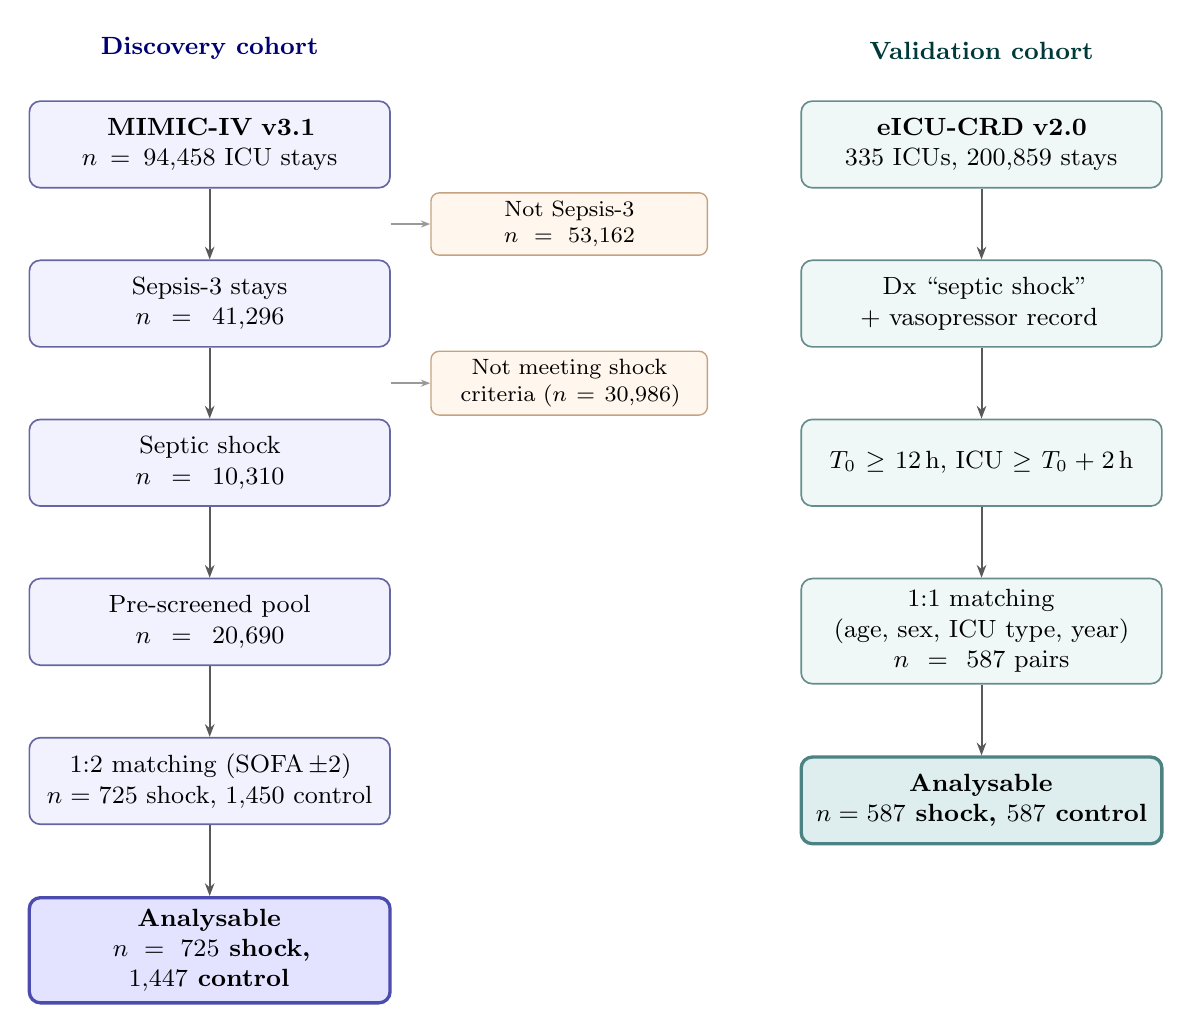
\begin{tikzpicture}[
    node distance = 9mm,
    %% Discovery column boxes
    mbox/.style = {
      draw=blue!40!black!60, line width=0.6pt,
      rounded corners=4pt, fill=blue!5,
      text width=43mm, align=center,
      font=\small, inner sep=4pt, minimum height=11mm},
    fbox/.style = {
      draw=blue!55!black!70, line width=1.2pt,
      rounded corners=4pt, fill=blue!11,
      text width=43mm, align=center,
      font=\small\bfseries, inner sep=4pt, minimum height=11mm},
    %% Validation column boxes
    vbox/.style = {
      draw=teal!50!black!60, line width=0.6pt,
      rounded corners=4pt, fill=teal!6,
      text width=43mm, align=center,
      font=\small, inner sep=4pt, minimum height=11mm},
    vfbox/.style = {
      draw=teal!60!black!70, line width=1.2pt,
      rounded corners=4pt, fill=teal!13,
      text width=43mm, align=center,
      font=\small\bfseries, inner sep=4pt, minimum height=11mm},
    %% Exclusion boxes (between columns, to the right of MIMIC arrows)
    excl/.style = {
      draw=orange!55!black!50, line width=0.5pt,
      rounded corners=3pt, fill=orange!7,
      text width=33mm, align=center,
      font=\footnotesize, inner sep=3pt},
    %% Arrows
    arr/.style  = {-{Stealth[scale=0.75]}, line width=0.7pt, black!65},
    harr/.style = {-{Stealth[scale=0.65]}, line width=0.5pt, black!40},
  ]

    %% ── MIMIC-IV column ────────────────────────────────────────────────────
    \node[mbox]              (M1) {\textbf{MIMIC-IV v3.1}\\$n = 94{,}458$ ICU stays};
    \node[mbox, below=of M1] (M2) {Sepsis-3 stays\\$n = 41{,}296$};
    \node[mbox, below=of M2] (M3) {Septic shock\\$n = 10{,}310$};
    \node[mbox, below=of M3] (M4) {Pre-screened pool\\$n = 20{,}690$};
    \node[mbox, below=of M4] (M5) {1:2 matching (SOFA\,$\pm$2)\\$n = 725$ shock, $1{,}450$ control};
    \node[fbox, below=of M5] (M6) {Analysable\\$n = 725$ shock, $1{,}447$ control};

    \draw[arr] (M1)--(M2); \draw[arr] (M2)--(M3);
    \draw[arr] (M3)--(M4); \draw[arr] (M4)--(M5); \draw[arr] (M5)--(M6);

    %% Exclusion boxes — between MIMIC and eICU columns
    \path (M1.south)--coordinate[midway](m12)(M2.north);
    \path (M2.south)--coordinate[midway](m23)(M3.north);
    \coordinate (XR) at ($(M1.east)+(5mm,0)$);
    \node[excl, anchor=west] (Ex1) at (XR|-m12) {Not Sepsis-3\\$n = 53{,}162$};
    \node[excl, anchor=west] (Ex2) at (XR|-m23) {Not meeting shock\\criteria ($n = 30{,}986$)};
    \draw[harr] (M1.east|-m12)--(Ex1.west);
    \draw[harr] (M2.east|-m23)--(Ex2.west);

    %% ── eICU-CRD column ─────────────────────────────────────────────────
    %% 52mm from MIMIC right edge clears excl boxes (5+33=38mm) with 14mm margin
    \node[vbox, right=52mm of M1] (V1) {\textbf{eICU-CRD v2.0}\\335 ICUs, $200{,}859$ stays};
    \node[vbox, below=of V1]      (V2) {Dx ``septic shock''\\+ vasopressor record};
    \node[vbox, below=of V2]      (V3) {$T_0 \geq 12$\,h, ICU $\geq T_0+2$\,h};
    \node[vbox, below=of V3]      (V4) {1:1 matching\\(age, sex, ICU type, year)\\$n = 587$ pairs};
    \node[vfbox, below=of V4]     (V5) {Analysable\\$n = 587$ shock, $587$ control};

    \draw[arr] (V1)--(V2); \draw[arr] (V2)--(V3);
    \draw[arr] (V3)--(V4); \draw[arr] (V4)--(V5);

    %% ── Column headers ─────────────────────────────────────────────────────
    \node[above=4mm of M1, font=\small\bfseries, text=blue!45!black]  {Discovery cohort};
    \node[above=4mm of V1, font=\small\bfseries, text=teal!45!black]   {Validation cohort};

    %% ── Dashed vertical separator ──────────────────────────────────────────
    %\coordinate (sep_top) at ($(M1.north east)!0.5!(V1.north west)+(0,4mm)$);
    %\coordinate (sep_bot) at ($(M6.south east)!0.5!(V5.south west)$);
    %\draw[dashed, black!18, line width=0.8pt] (sep_top)--(sep_bot);

  \end{tikzpicture}
  \caption{Study flow diagram.
  \textbf{Left} (blue): MIMIC-IV v3.1 discovery cohort.
  From 94,458 ICU stays, 41,296 met Sepsis-3 criteria; 10,310 further
  met the operational septic shock definition (vasopressor\,$\geq$1\,h,
  lactate\,$>$2, crystalloid\,$\geq$1\,L); 2,172 observations were
  analysable after 1:2 risk-set matching and time-series cleaning
  (725 shock, 1,447 control).
  Exclusion boxes (orange, left) show filtering steps.
  \textbf{Right} (teal): eICU-CRD v2.0 external validation cohort.
  A surrogate definition (diagnosis string + vasopressor record) was
  applied across 335 ICUs; after eligibility filtering and 1:1 matching,
  587 matched pairs across 163 hospitals were analysable.}
  \label{fig:consort}
\end{figure}

\clearpage

% Fig 2a: AC1 + MAP variance timeseries
\begin{figure}[htbp]
  \centering
  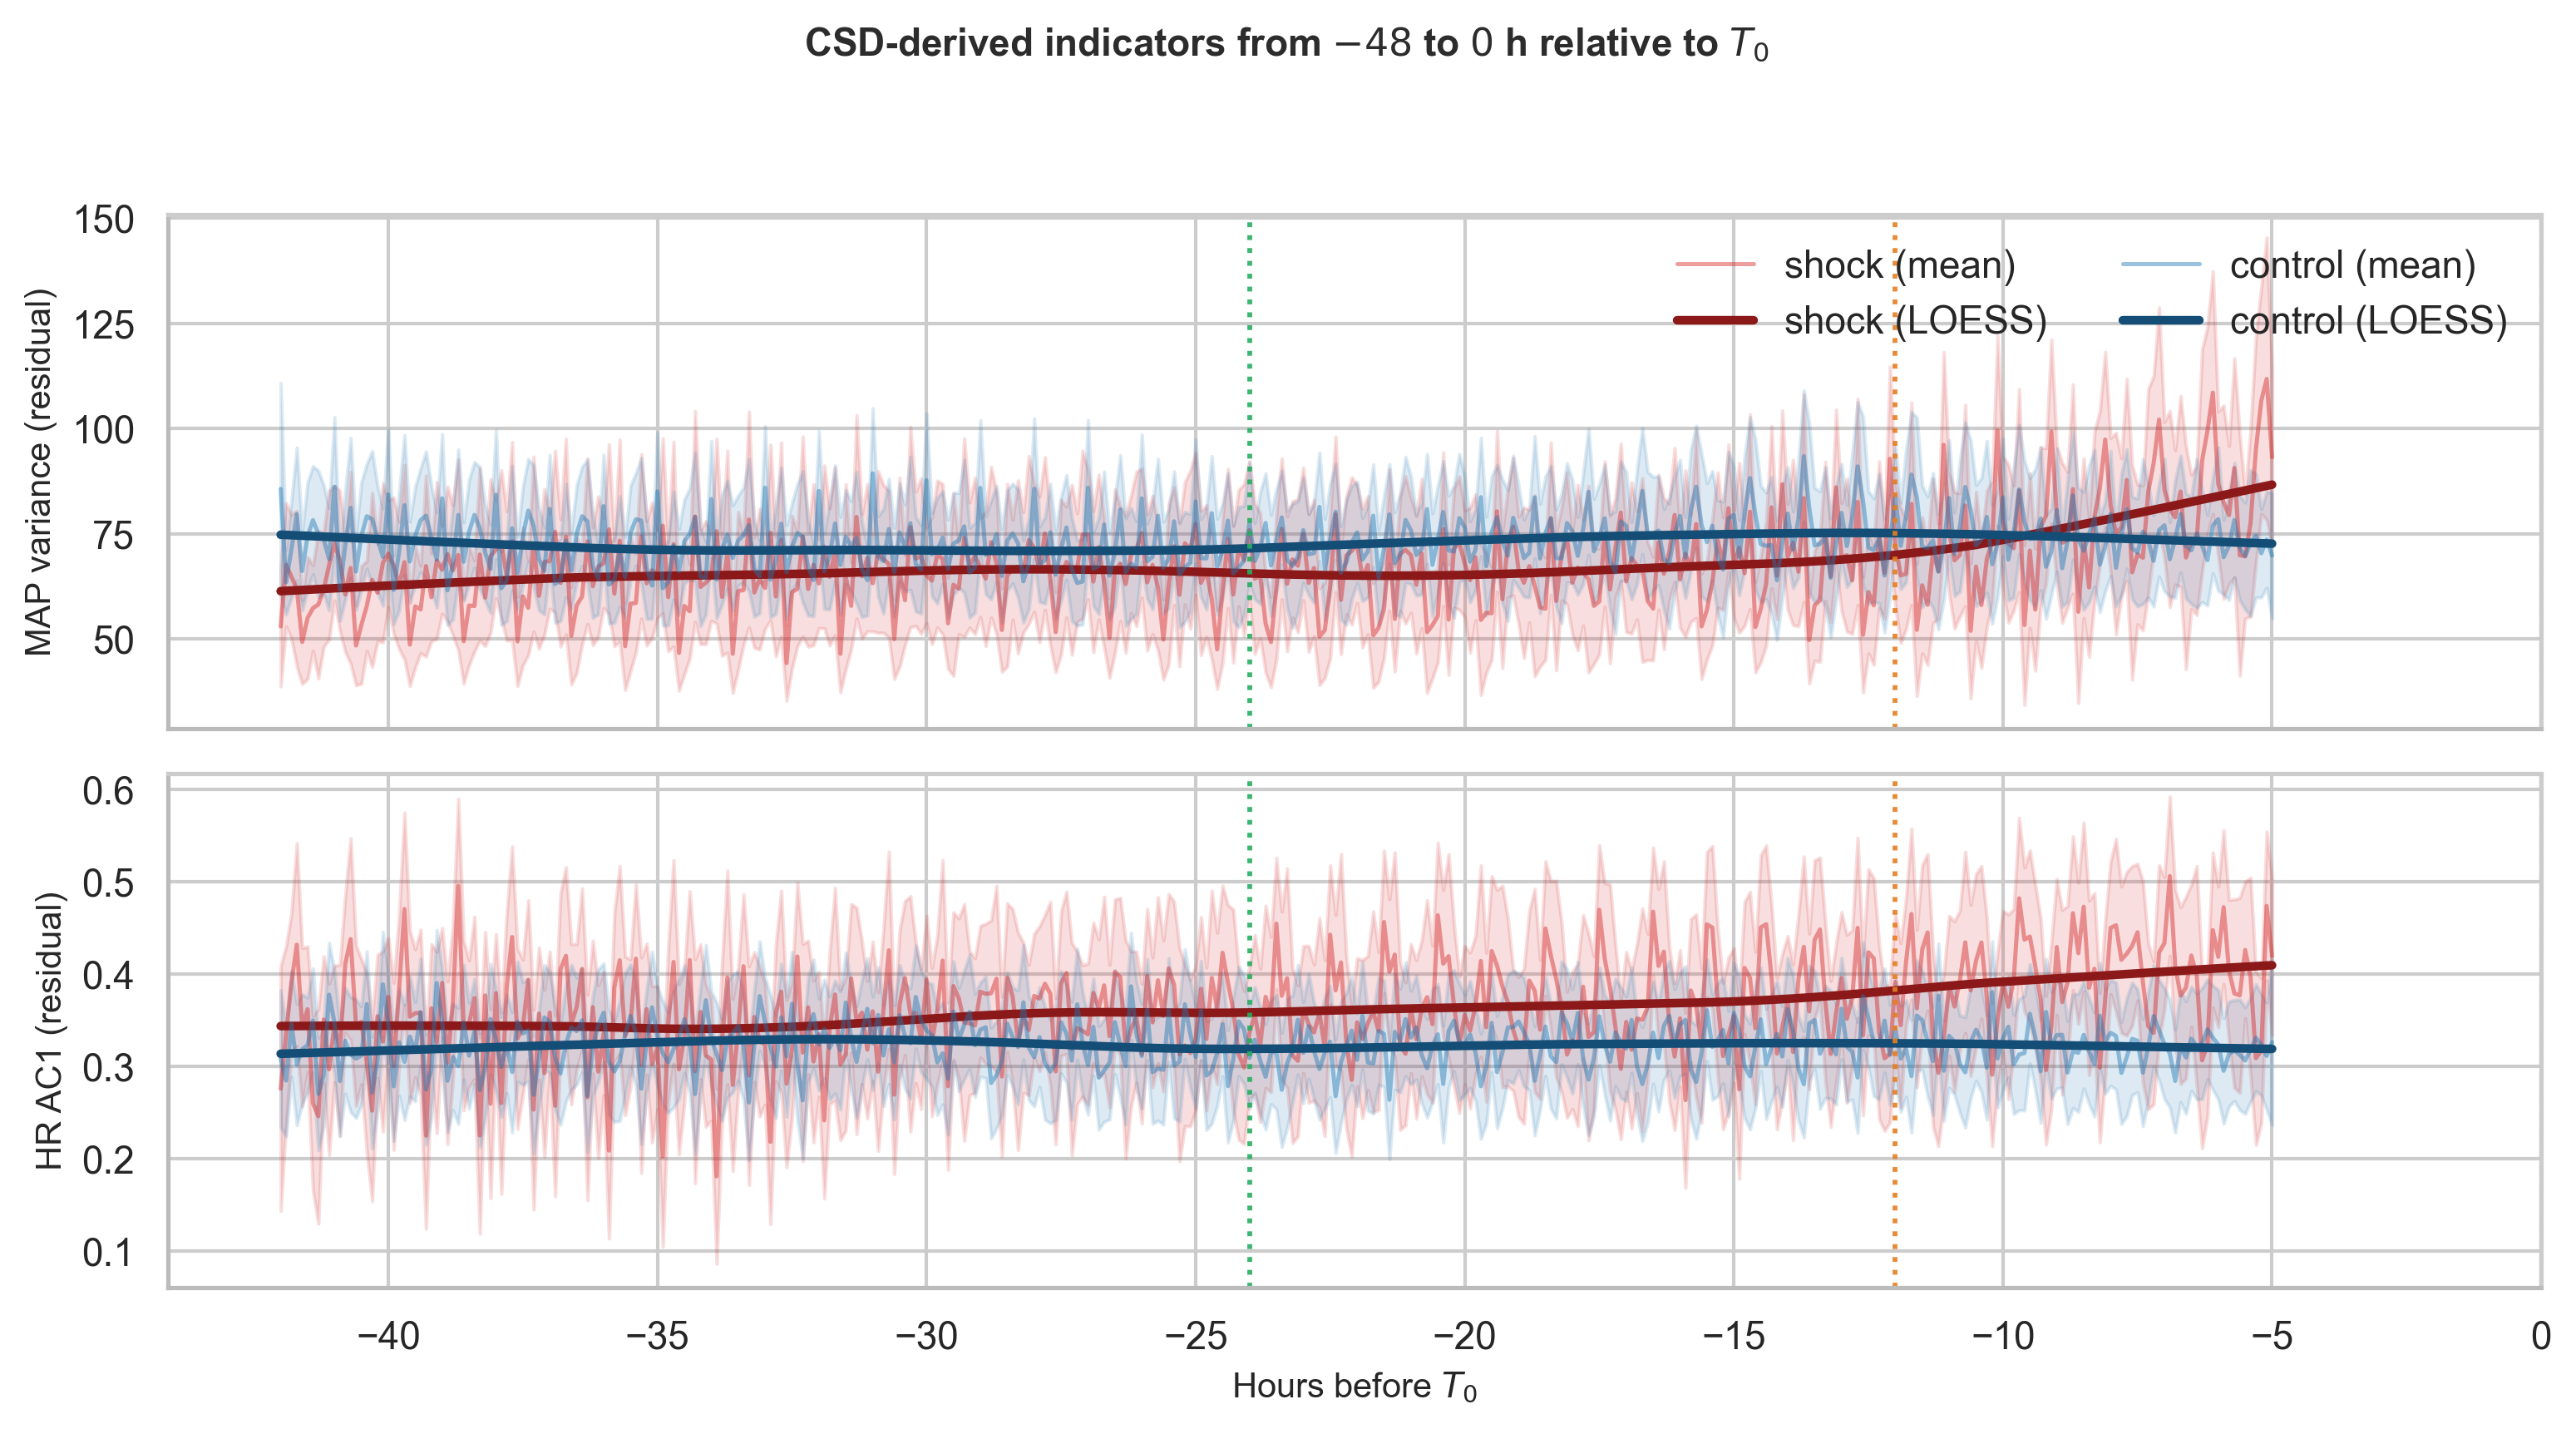
\includegraphics[width=\textwidth]{figures/fig2a_ac1_timeseries.png}
  \caption{CSD-derived indicators from $-48$ to $0$\,h relative to \Tzero\
  (MIMIC-IV).
  Mean~$\pm$~95\,\% CI (shaded); LOESS trend (solid).
  Green dotted: early/late boundary ($-24$\,h);
  orange dotted: late-window start ($-12$\,h);
  grey dashed: \Tzero.
  HR AC1 diverges in the late-window phase; MAP variance shows no
  consistent group separation.}
  \label{fig:ts-ac1}
\end{figure}

\clearpage

% Fig 2b: Topological indicators timeseries
\begin{figure}[htbp]
  \centering
  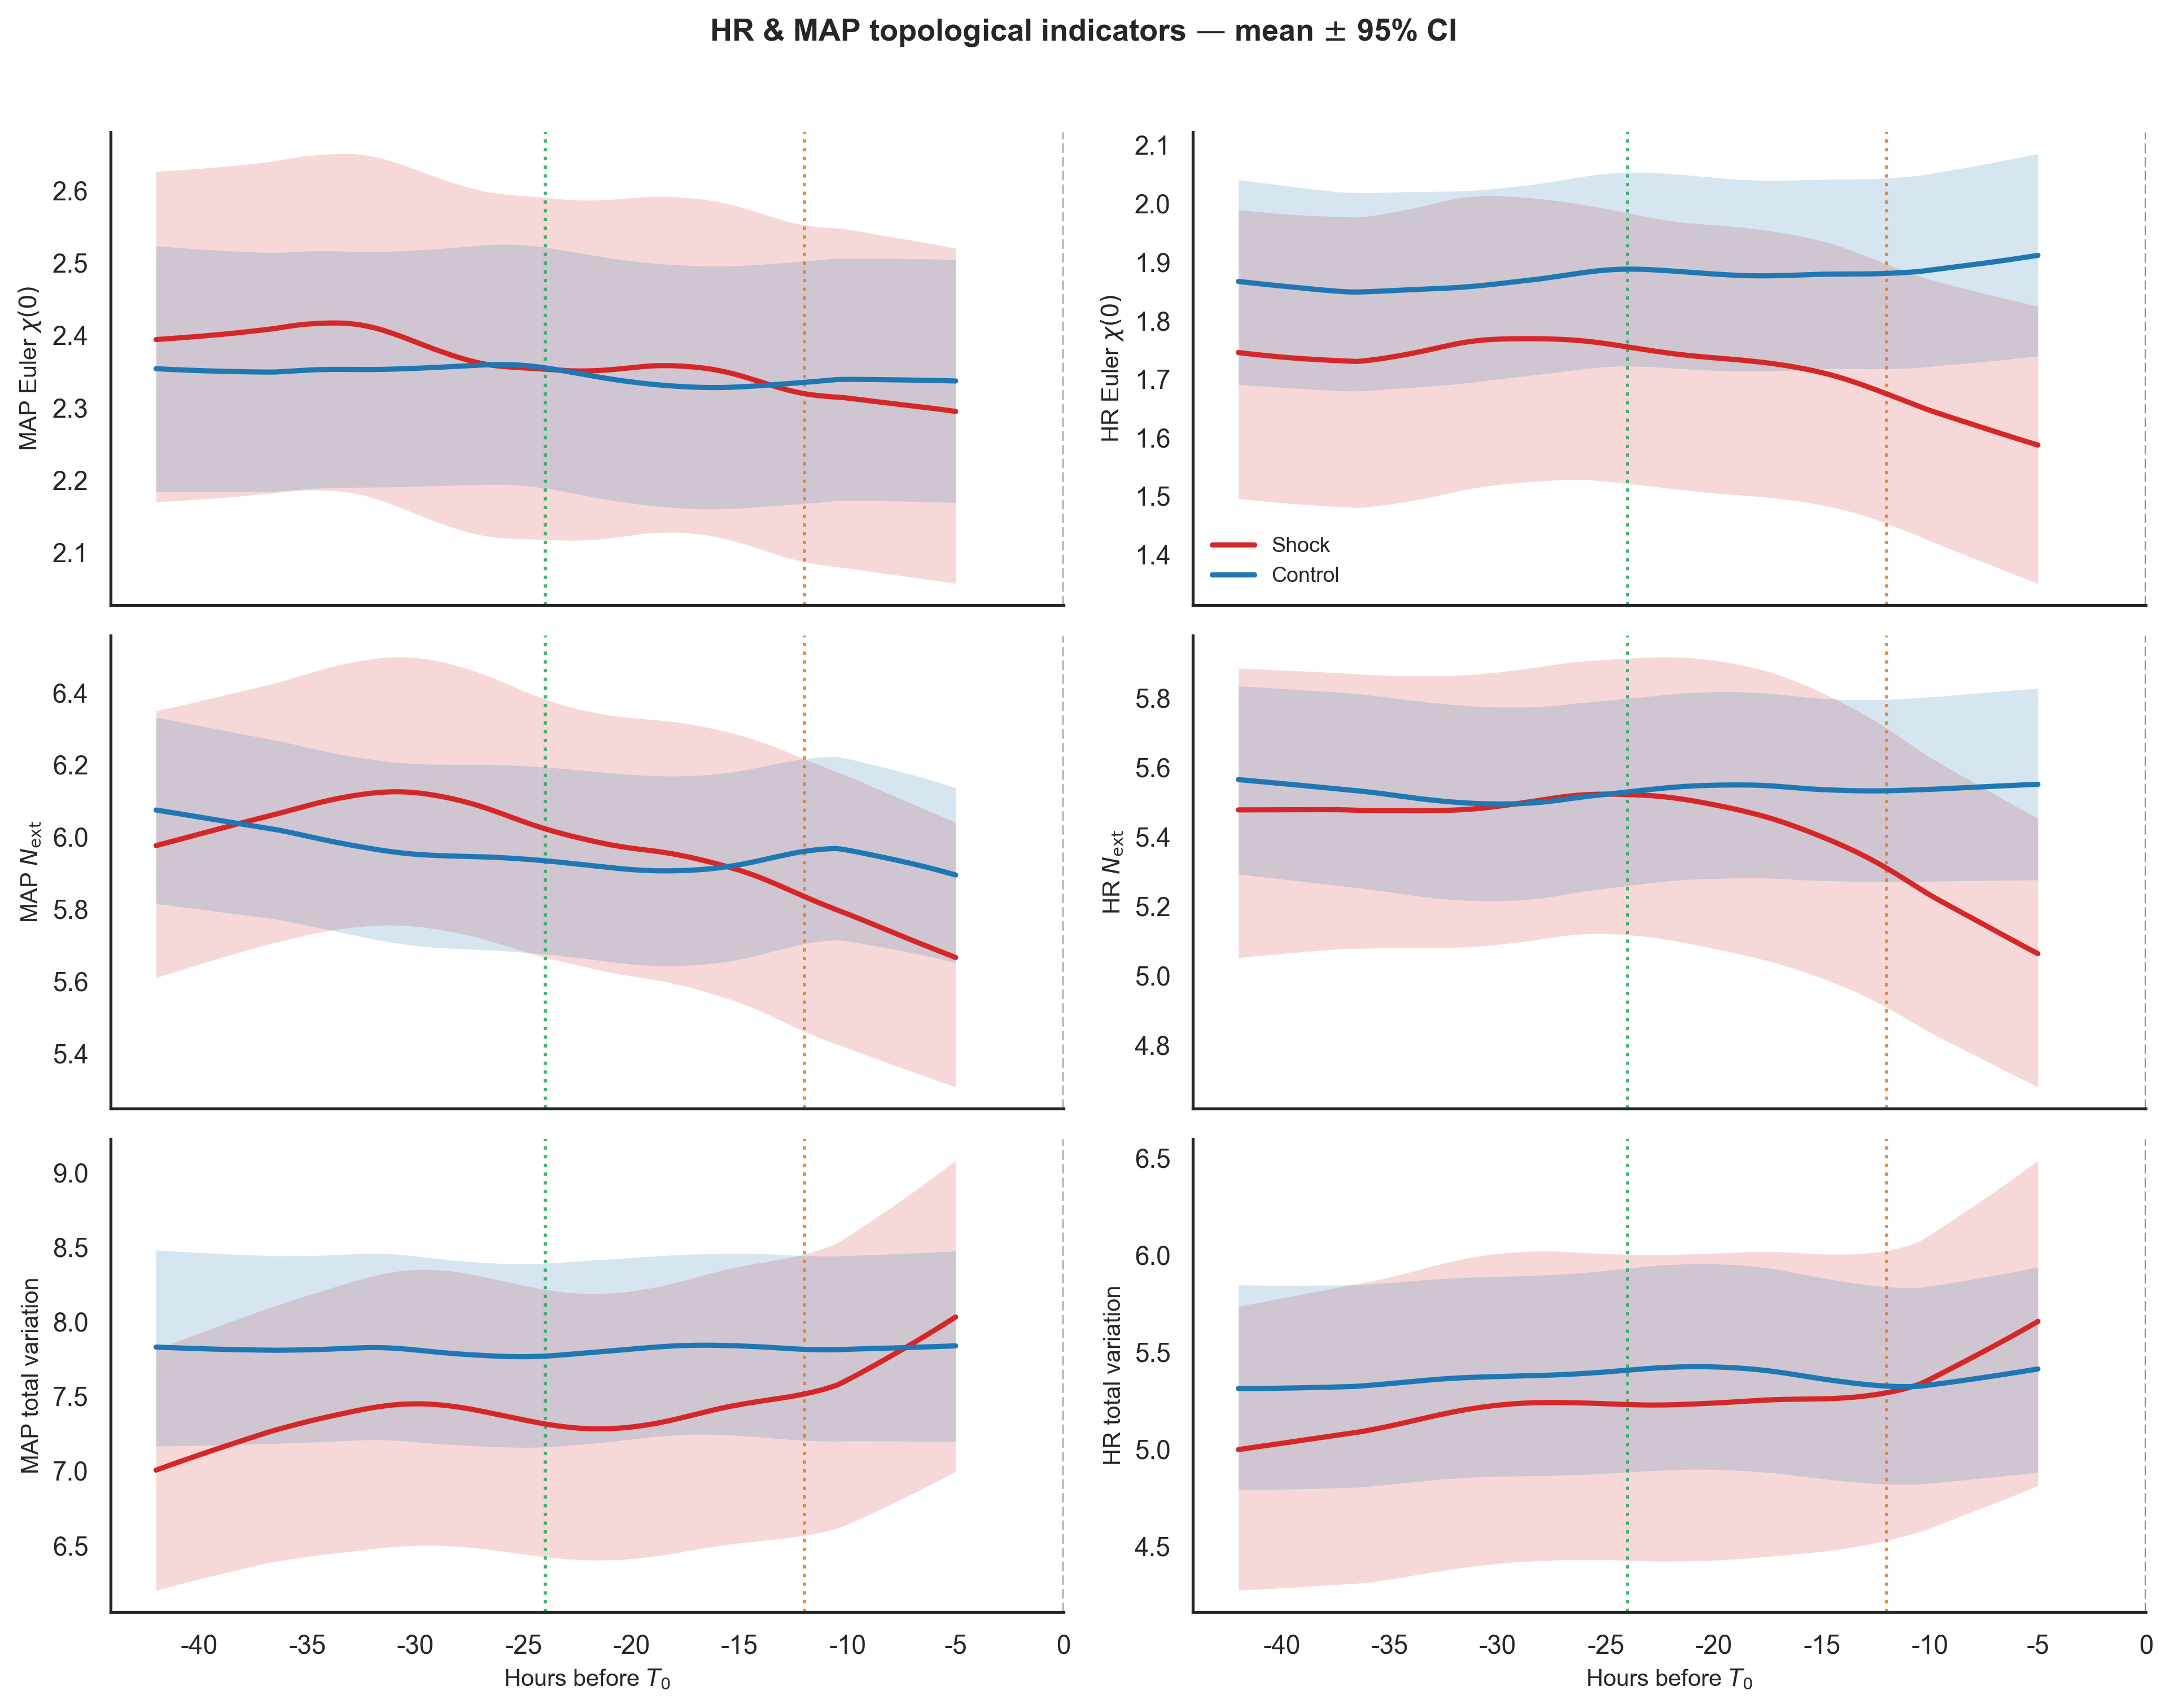
\includegraphics[width=\textwidth]{figures/fig2b_euler_timeseries.png}
  \caption{Topological indicators from $-48$ to $0$\,h relative to \Tzero\
  (MIMIC-IV).
  HR \chihr\ and HR \Nextreme\ decline progressively in the shock group
  from $\approx -24$\,h; MAP indicators and normalised total variation
  show no consistent divergence.
  Format as in Figure~\ref{fig:ts-ac1}.}
  \label{fig:ts-euler}
\end{figure}

\clearpage

% Fig 3: Four-indicator forest plot (M1/S1/S2)
\begin{figure}[htbp]
  \centering
  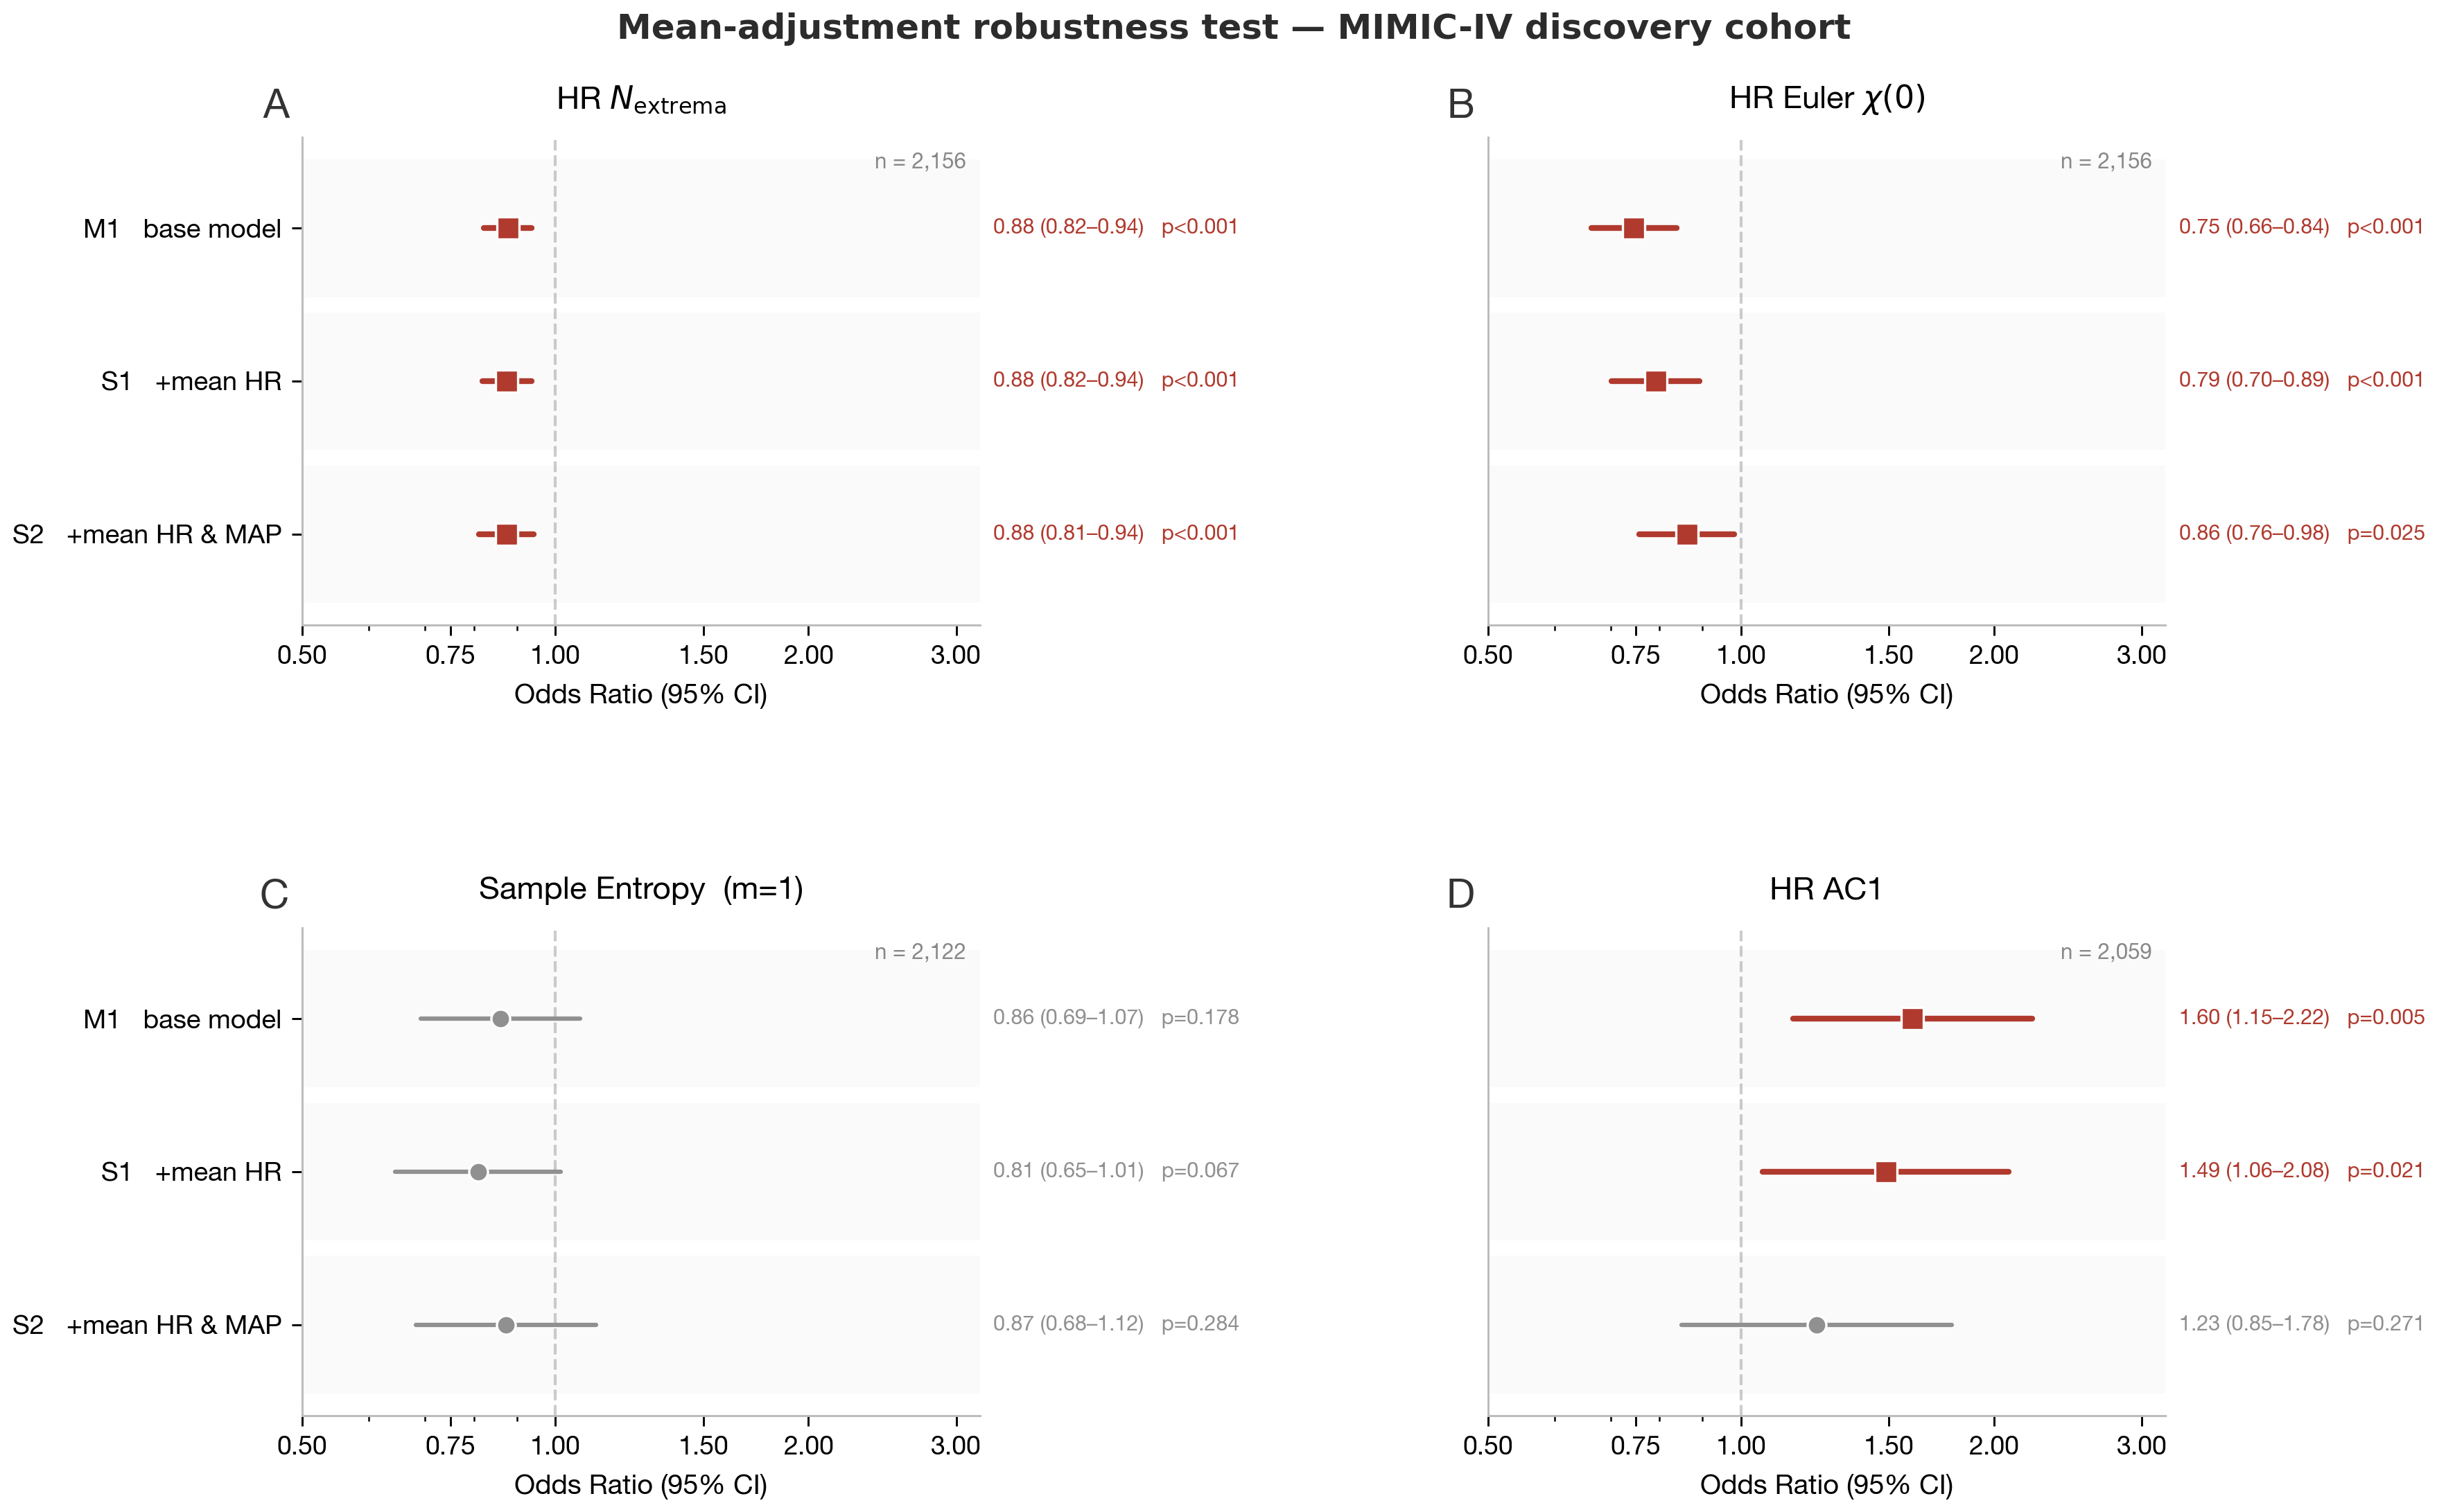
\includegraphics[width=\textwidth]{figures/fig3_forest.png}
  \caption{Four-indicator comparison across M1 (base), S1 (+mean HR),
  and S2 (+mean HR and MAP) model specifications (MIMIC-IV discovery cohort).
  Panels show OR (95\,\%\,CI) for HR \Nextreme\ (top left),
  HR \chihr\ (top right),
  SampEn $m=1$, $r=0.5\sigma_{48}$ (bottom left),
  and HR AC1 (bottom right).
  Red symbols: $p<0.05$; grey: $p\geq0.05$.
  \Nextreme\ is the only indicator that remains significant across all three
  model specifications.}
  \label{fig:forest}
\end{figure}

\clearpage

% Fig 4: eICU T0-stratified sensitivity
\begin{figure}[htbp]
  \centering
  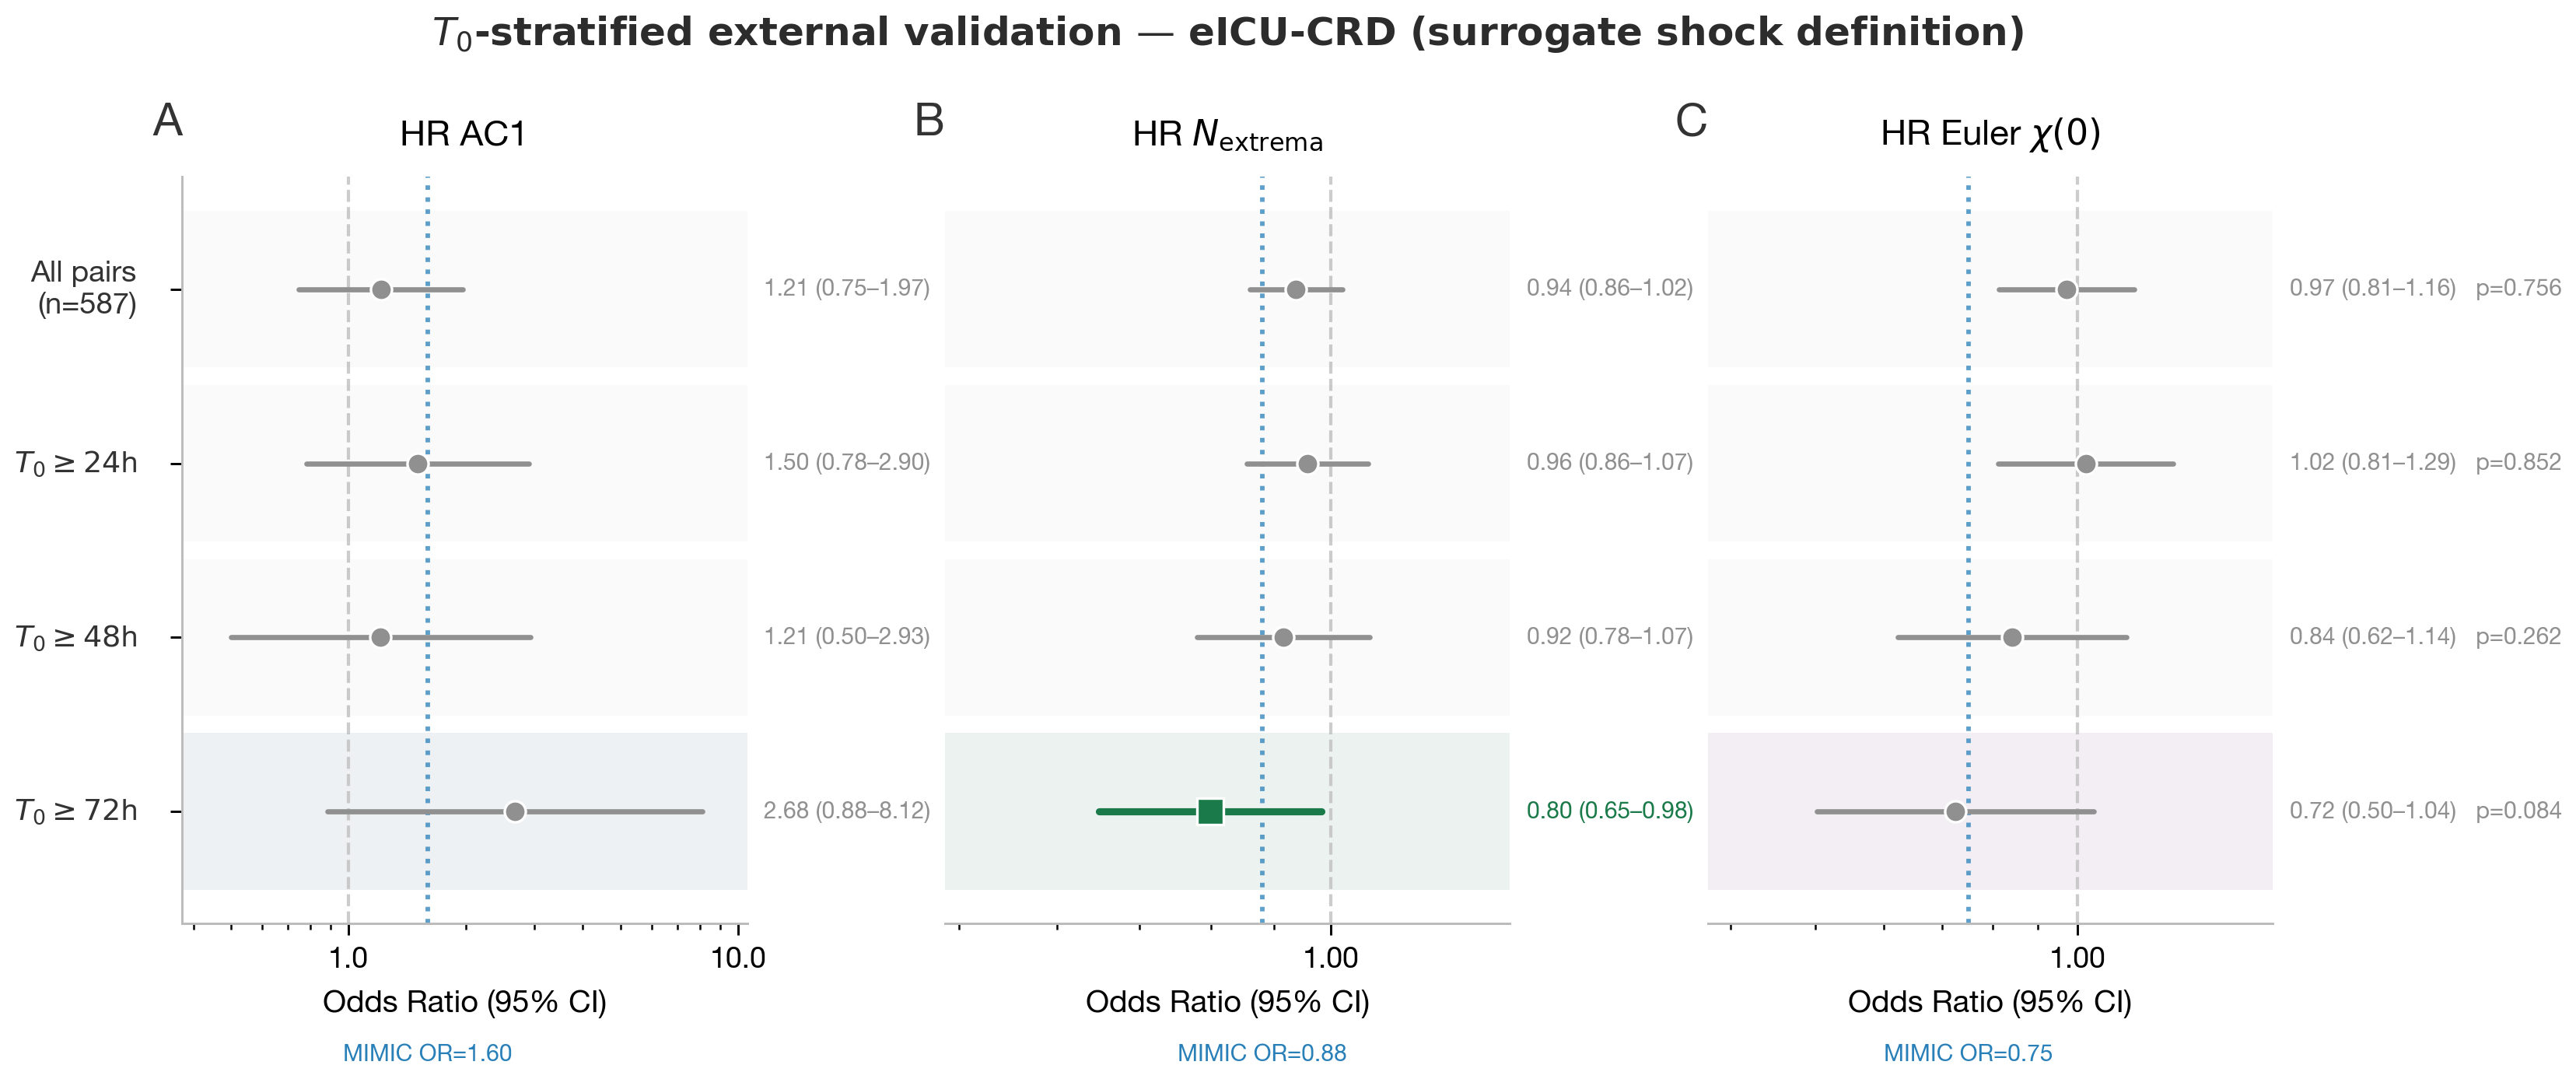
\includegraphics[width=0.85\textwidth]{figures/fig4_t0strat.png}
  \caption{$T_0$-stratified external validation in eICU-CRD.
  OR (95\,\%\,CI) for \Nextreme\ across $T_0$ thresholds (full cohort,
  $\geq$24, $\geq$48, $\geq$72\,h).
  Statistical significance ($p<0.05$) emerges at $T_0\geq 72$\,h
  (103 pairs), consistent with the observation that adequate pre-event
  exposure is required to distinguish oscillatory complexity differences.
  This analysis is post-hoc and exploratory.}
  \label{fig:t0strat}
\end{figure}

\clearpage

% Fig 5: Euler vs AC1 full sensitivity forest
\begin{figure}[htbp]
  \centering
  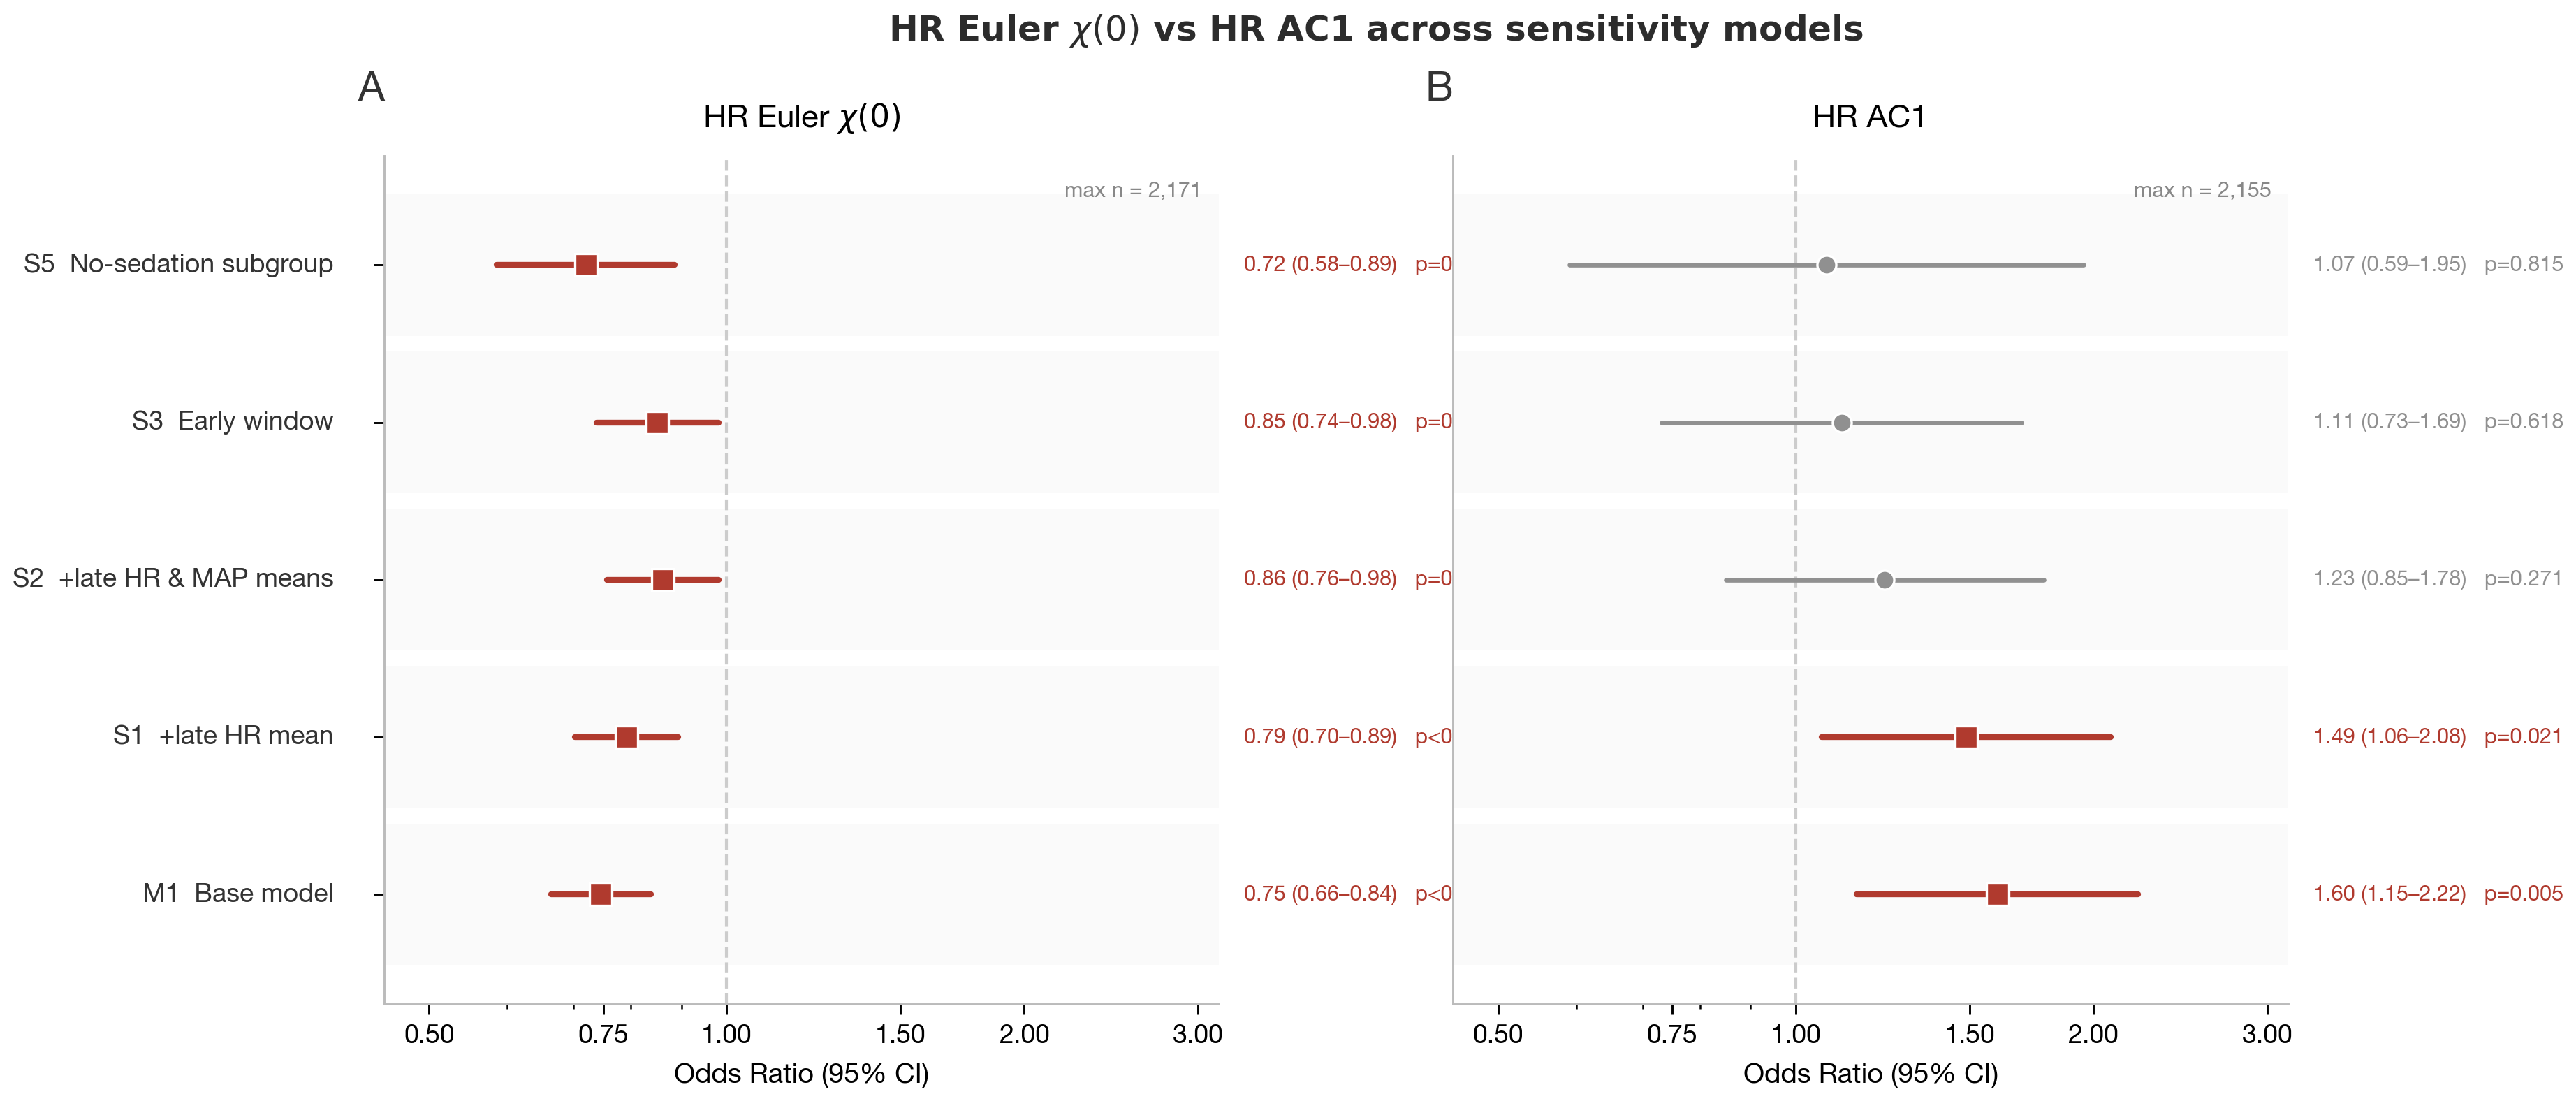
\includegraphics[width=\textwidth]{figures/fig5_vs_ac1_forest.png}
  \caption{Forest plot comparing OR (95\,\%\,CI) for HR \chihr\ (left)
  and HR AC1 (right) across corresponding model specifications.
  Red symbols: $p<0.05$; grey: $p\geq0.05$.
  The key divergence is in S2: \chihr\ retains significance after
  adjustment for both late-window mean HR and MAP, whereas AC1 does not.}
  \label{fig:vs-ac1-forest}
\end{figure}

% ================================================================
% TABLES
% ================================================================
\clearpage

% Table 1: Baseline characteristics
\begin{table}[htbp]
  \centering
  \caption{Baseline characteristics of the MIMIC-IV matched cohort
  (725 shock, 1,447 controls).
  Continuous variables: median (IQR); categorical: $n$ (\%).
  Standardised mean differences (SMD) computed within matched pairs.}
  \label{tab:baseline}
  \small
  \begin{tabular}{lrrr}
    \toprule
    \textbf{Characteristic} & \textbf{Shock ($n=725$)} &
    \textbf{Control ($n=1{,}447$)} & \textbf{SMD} \\
    \midrule
    \multicolumn{4}{l}{\textit{Demographics}} \\
    Age, years            & 65 [54--74] & 63 [54--75] & 0.035 \\
    Male sex              & 411 (56.7\%) & 862 (59.6\%) & $-$0.058 \\
    \midrule
    \multicolumn{4}{l}{\textit{Severity and ICU course}} \\
    Admission SOFA        & 6 [4--9] & 6 [4--8] & 0.045 \\
    ICU LOS, days         & 13.8 [8.8--22.2] & 12.3 [7.7--19.6] & 0.144 \\
    Hospital mortality    & 412 (56.8\%) & 308 (21.3\%) & 0.782 \\
    \midrule
    \multicolumn{4}{l}{\textit{Treatment at \Tzero}} \\
    Respiratory support   & 630 (86.9\%) & 1{,}220 (84.3\%) & 0.074 \\
    Vasopressor before \Tzero & 676 (93.2\%) & 599 (41.4\%) & 1.326 \\
    \midrule
    \multicolumn{4}{l}{\textit{ICU type (first care unit)}} \\
    MICU                  & 351 (48.4\%) & 627 (43.3\%) & 0.102 \\
    SICU                  & 177 (24.4\%) & 456 (31.5\%) & $-$0.159 \\
    CCU/CSRU              & 162 (22.3\%) & 217 (15.0\%) & 0.189 \\
    Neuro/NICU            & 14 (1.9\%)  & 117 (8.1\%)  & $-$0.285 \\
    Other                 & 21 (2.9\%)  & 30 (2.1\%)  & 0.053 \\
    \midrule
    \multicolumn{4}{l}{\textit{Monitoring modality}} \\
    ABP-dominant          & 280 (38.6\%) & 543 (37.5\%) & 0.023 \\
    NBP-dominant          & 359 (49.5\%) & 738 (51.0\%) & $-$0.030 \\
    Mixed                 & 86 (11.9\%) & 166 (11.5\%) & 0.012 \\
    \bottomrule
  \end{tabular}
  \vspace{2pt}\\
  \raggedright\footnotesize
  Continuous variables: median [IQR]; categorical: $n$ (\%).
  $|\text{SMD}| \geq 0.1$ indicates meaningful imbalance.
\end{table}

\clearpage

% Table 2: GEE between-group comparison (all indicators)
\begin{table}[htbp]
  \centering
  \caption{Between-group comparisons of early-warning indicators
  (GEE, Gaussian family, exchangeable correlation, \texttt{stay\_id}
  clustering; Holm--Bonferroni correction across all 18 tests).
  Values are group means.}
  \label{tab:gee}
  \small
  \resizebox{\textwidth}{!}{%
  \begin{tabular}{lcccccccccc}
    \toprule
    & \multicolumn{3}{c}{\textbf{Early window}} & \multicolumn{3}{c}{\textbf{Late window}} & \multicolumn{3}{c}{\textbf{$\Delta$ (late$-$early)}} \\
    \cmidrule(lr){2-4}\cmidrule(lr){5-7}\cmidrule(lr){8-10}
    \textbf{Indicator} & Shock & Control & Holm $p$ & Shock & Control & Holm $p$ & Shock & Control & Holm $p$ \\
    \midrule
    HR AC1              & 0.345 & 0.323 & 0.316   & 0.382 & 0.323 & $<$0.001 & $+$0.036 & $-$0.002 & 0.187 \\
    MAP variance        & 64.2  & 72.3  & 0.069   & 77.0  & 75.0  & 1.000    & $+$12.8  & $+$2.4   & 0.025 \\
    HR $\chi(0)$        & 1.75  & 1.86  & 0.020   & 1.62  & 1.89  & $<$0.001 & $-$0.131 & $+$0.030 & 0.013 \\
    HR $N_{\text{ext}}$ & 5.48  & 5.52  & 1.000   & 5.16  & 5.53  & $<$0.001 & $-$0.315 & $+$0.020 & $<$0.001 \\
    MAP $\chi(0)$       & 2.39  & 2.35  & 1.000   & 2.28  & 2.33  & 1.000    & $-$0.107 & $-$0.017 & 0.446 \\
    MAP $N_{\text{ext}}$& 6.06  & 5.98  & 0.723   & 5.73  & 5.92  & 0.051    & $-$0.338 & $-$0.066 & 0.012 \\
    \midrule
    \multicolumn{10}{l}{\textit{LMM time$\times$group interaction}} \\
    HR AC1: $\beta=+0.0014$, $p=0.024$ &
    \multicolumn{3}{l}{HR $\chi(0)$: $\beta=-0.0053$, $p=0.006$} &
    \multicolumn{3}{l}{HR $N_{\text{ext}}$: $\beta=-0.0090$, $p=0.004$} &
    \multicolumn{3}{l}{MAP: all $p>0.05$} \\
    \bottomrule
  \end{tabular}}
\end{table}

\clearpage

% Table 3: Conditional logistic regression (all indicators, M1-S5)
\begin{table}[htbp]
  \centering
  \caption{Conditional logistic regression results (stratified by matched
  pair; MIMIC-IV).
  Models: M1 base; S1 +late mean HR; S2 +late mean HR and MAP;
  S3 early window; S5 no-sedation subgroup.
  All models include: invasive ventilation, beta-blocker, ICU type,
  monitoring modality (sedative omitted in S5).}
  \label{tab:logit}
  \small
  \begin{tabular}{llccc}
    \toprule
    \textbf{Model} & \textbf{Predictor} & \textbf{$N$} &
    \textbf{OR (95\,\%\,CI)} & \textbf{$p$} \\
    \midrule
    \multicolumn{5}{l}{\textit{$N_{\text{extrema}}$ (primary topological indicator)}} \\
    M1 Base model            & $N_{\text{extrema}}$ late  & 2{,}156 & 0.88 (0.82--0.94) & $<$0.001 \\
    S1 + late mean HR        & $N_{\text{extrema}}$ late  & 2{,}156 & 0.88 (0.82--0.94) & $<$0.001 \\
    S2 + late mean HR \& MAP & $N_{\text{extrema}}$ late  & 2{,}138 & 0.87 (0.81--0.94) & $<$0.001 \\
    S5 No-sedation           & $N_{\text{extrema}}$ late  &   544 & 0.79 (0.67--0.93) & 0.004 \\
    \midrule
    \multicolumn{5}{l}{\textit{Euler $\chi_{\text{HR}}(0)$ (secondary topological indicator)}} \\
    M1 Base model            & $\chi_{\text{HR}}(0)$ late  & 2{,}156 & 0.75 (0.66--0.84) & $<$0.001 \\
    S1 + late mean HR        & $\chi_{\text{HR}}(0)$ late  & 2{,}156 & 0.79 (0.70--0.89) & $<$0.001 \\
    S2 + late mean HR \& MAP & $\chi_{\text{HR}}(0)$ late  & 2{,}138 & 0.86 (0.76--0.98) & 0.025 \\
    S3 Early window$^a$      & $\chi_{\text{HR}}(0)$ early & 2{,}171 & 0.85 (0.74--0.98) & 0.027 \\
    S5 No-sedation           & $\chi_{\text{HR}}(0)$ late  &   544 & 0.72 (0.58--0.89) & 0.002 \\
    \midrule
    \multicolumn{5}{l}{\textit{SampEn ($m=1$, $r=0.5\sigma_{48}$)}} \\
    M1 Base model            & SampEn late  & 2{,}122 & 0.86 (0.69--1.07) & 0.178 \\
    S1 + late mean HR        & SampEn late  & 2{,}122 & 0.81 (0.64--1.02) & 0.067 \\
    S2 + late mean HR \& MAP & SampEn late  & 2{,}104 & 0.87 (0.68--1.12) & 0.284 \\
    \midrule
    \multicolumn{5}{l}{\textit{HR AC1 (CSD comparator)}} \\
    M1 Base model            & AC1 late  & 2{,}059 & 1.60 (1.15--2.22) & 0.005 \\
    S1 + late mean HR        & AC1 late  & 2{,}059 & 1.49 (1.06--2.08) & 0.021 \\
    S2 + late mean HR \& MAP & AC1 late  & 2{,}041 & 1.23 (0.85--1.78) & 0.271 \\
    S3 Early window$^a$      & AC1 early & 2{,}155 & 1.11 (0.73--1.69) & 0.618 \\
    S5 No-sedation           & AC1 late  &   526 & 1.07 (0.59--1.95) & 0.815 \\
    \bottomrule
  \end{tabular}
  \vspace{2pt}\\
  \raggedright\footnotesize
  $^a$ S3 additionally adjusts for early-window raw mean HR and MAP.
  All models include: invasive ventilation, sedative exposure (omitted in S5),
  beta-blocker exposure, ICU type, and monitoring modality.
  Admission SOFA conditioned out by matched-pair likelihood.
\end{table}

\clearpage

% Table 4: eICU T0-stratified validation
\begin{table}[htbp]
  \centering
  \caption{External validation: $T_0$-stratified conditional logistic
  regression in eICU-CRD (1:1 matched cohort).
  MIMIC-IV row shown for reference (M1 specification).
  $T_0$-stratified analysis is post-hoc exploratory.}
  \label{tab:eicu}
  \small
  \resizebox{\textwidth}{!}{%
  \begin{tabular}{lcccccccc}
    \toprule
    & \multicolumn{2}{c}{\textbf{\Nextreme}}
    & \multicolumn{2}{c}{\textbf{\chihr}}
    & \multicolumn{2}{c}{\textbf{SampEn}}
    & \multicolumn{2}{c}{\textbf{AC1}} \\
    \cmidrule(lr){2-3}\cmidrule(lr){4-5}\cmidrule(lr){6-7}\cmidrule(lr){8-9}
    \textbf{Subset ($N$ pairs)} & OR (95\%CI) & $p$ & OR (95\%CI) & $p$
    & OR (95\%CI) & $p$ & OR (95\%CI) & $p$ \\
    \midrule
    \multicolumn{9}{l}{\textit{eICU-CRD}} \\
    Full cohort (587) & 0.94 (0.86--1.02) & 0.142 & 0.97 (0.81--1.16) & 0.756
    & 1.00 (0.76--1.31) & 0.978 & 1.21 (0.75--1.97) & 0.435 \\
    $T_0\geq 24$\,h (297) & 0.96 (0.86--1.07) & 0.455 & 1.02 (0.81--1.29) & 0.852
    & 1.04 (0.72--1.52) & 0.819 & 1.50 (0.78--2.90) & 0.224 \\
    $T_0\geq 48$\,h (154) & 0.92 (0.78--1.07) & 0.281 & 0.84 (0.62--1.14) & 0.262
    & 1.14 (0.67--1.96) & 0.628 & 1.21 (0.50--2.93) & 0.673 \\
    $T_0\geq 72$\,h (103)$^\star$ & \textbf{0.80 (0.65--0.98)} & \textbf{0.034}
    & 0.72 (0.50--1.04) & 0.084 & 1.17 (0.62--2.21) & 0.625
    & 2.68 (0.88--8.12) & 0.082 \\
    \midrule
    \multicolumn{9}{l}{\textit{MIMIC-IV (reference)}} \\
    Full cohort (725) & 0.88 (0.82--0.94) & $<$0.001 & 0.75 (0.66--0.84) & $<$0.001
    & 0.86 (0.69--1.07) & 0.178 & 1.60 (1.15--2.22) & 0.005 \\
    \bottomrule
  \end{tabular}}
  \vspace{2pt}\\
  \raggedright\footnotesize
  $^\star$ Post-hoc exploratory; interpret with caution.
  Severity-adjusted sensitivity ($T_0\geq72$\,h): $N_{\text{extrema}}$
  remained significant after adding SOFA non-cardiovascular
  (OR\,=\,0.80, $p=0.041$) and APACHE-IVa (OR\,=\,0.77, $p=0.038$);
  see Table~\ref{tab:sofa}.
\end{table}

% ================================================================
% SUPPLEMENTARY MATERIAL
% ================================================================
\clearpage
\appendix
\renewcommand{\thefigure}{S\arabic{figure}}
\renewcommand{\thetable}{S\arabic{table}}
\setcounter{figure}{0}
\setcounter{table}{0}

\section*{Supplementary Material}

% Fig S1: Perturbation-recovery Turn event analysis
\begin{figure}[htbp]
  \centering
  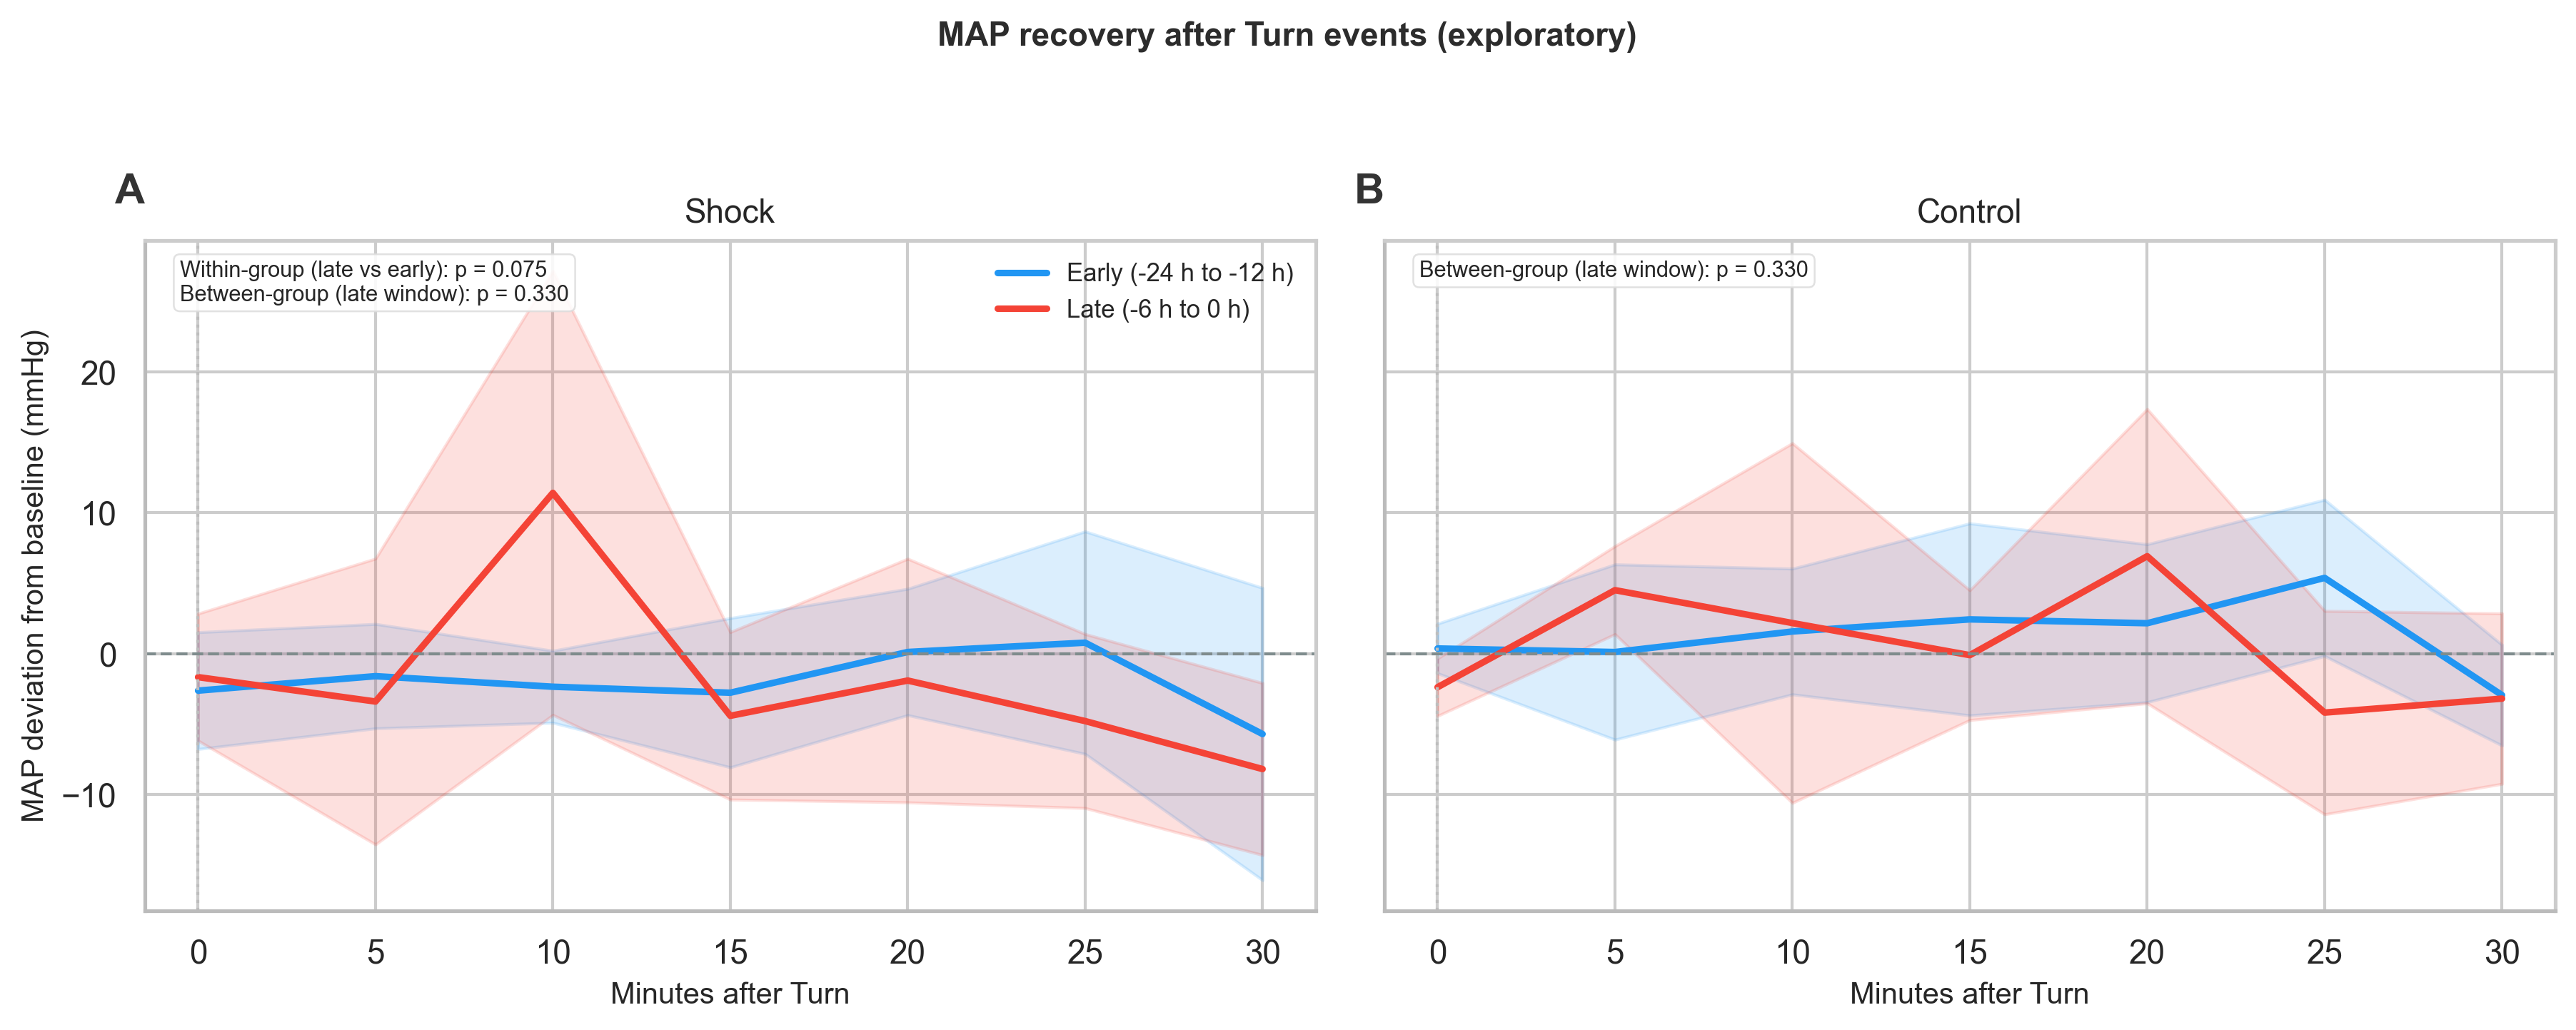
\includegraphics[width=0.85\textwidth]{figures/figS1_recovery.png}
  \caption{Perturbation-recovery analysis using nursing Turn events.
  660 Turn events identified in 330 patients.
  MAP area under the recovery curve did not differ significantly
  between early and late windows within the shock group ($p=0.075$)
  nor between shock and control groups ($p=0.330$).
  Hourly EHR resolution precludes reliable characterisation of
  perturbation-recovery curves, motivating the indirect structural
  complexity approach.}
  \label{fig:recovery}
\end{figure}

% Fig S2: Monitoring modality subgroup
\begin{figure}[htbp]
  \centering
  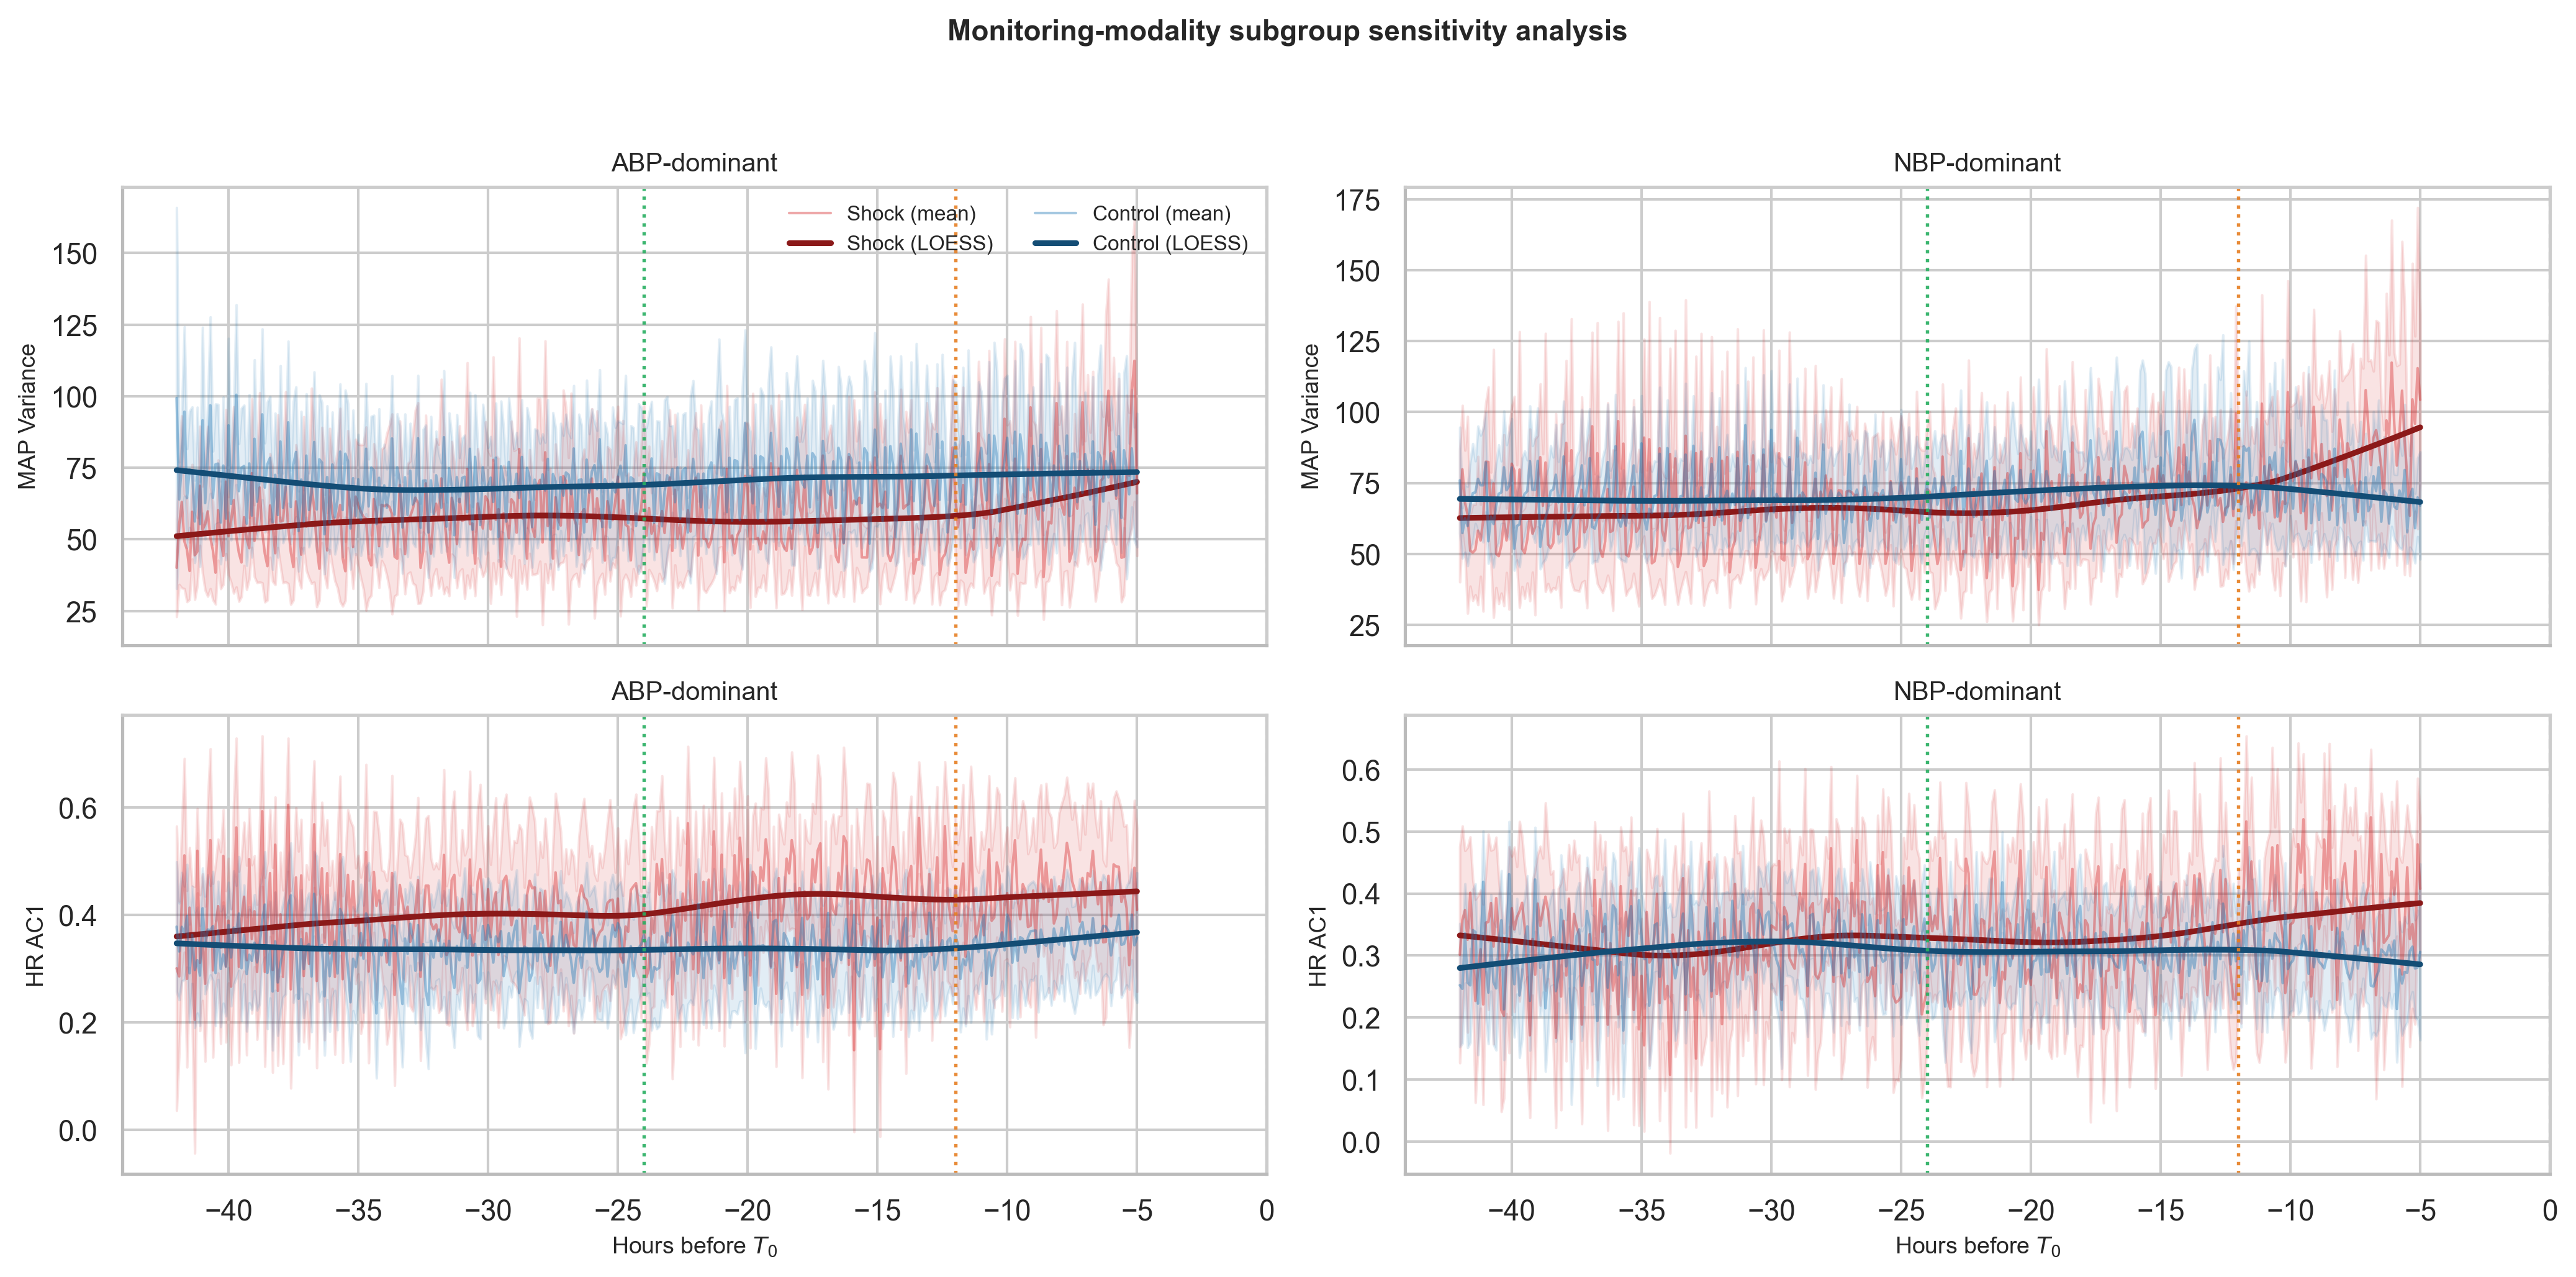
\includegraphics[width=\textwidth]{figures/figS2_subgroup.png}
  \caption{Monitoring modality subgroup sensitivity analysis (MIMIC-IV).
  HR AC1 and topological indicators stratified by arterial line vs
  non-invasive monitoring.}
  \label{fig:subgroup}
\end{figure}

% Fig S3: Delta (late-early) boxplots
\begin{figure}[htbp]
  \centering
  \begin{subfigure}[b]{0.48\textwidth}
    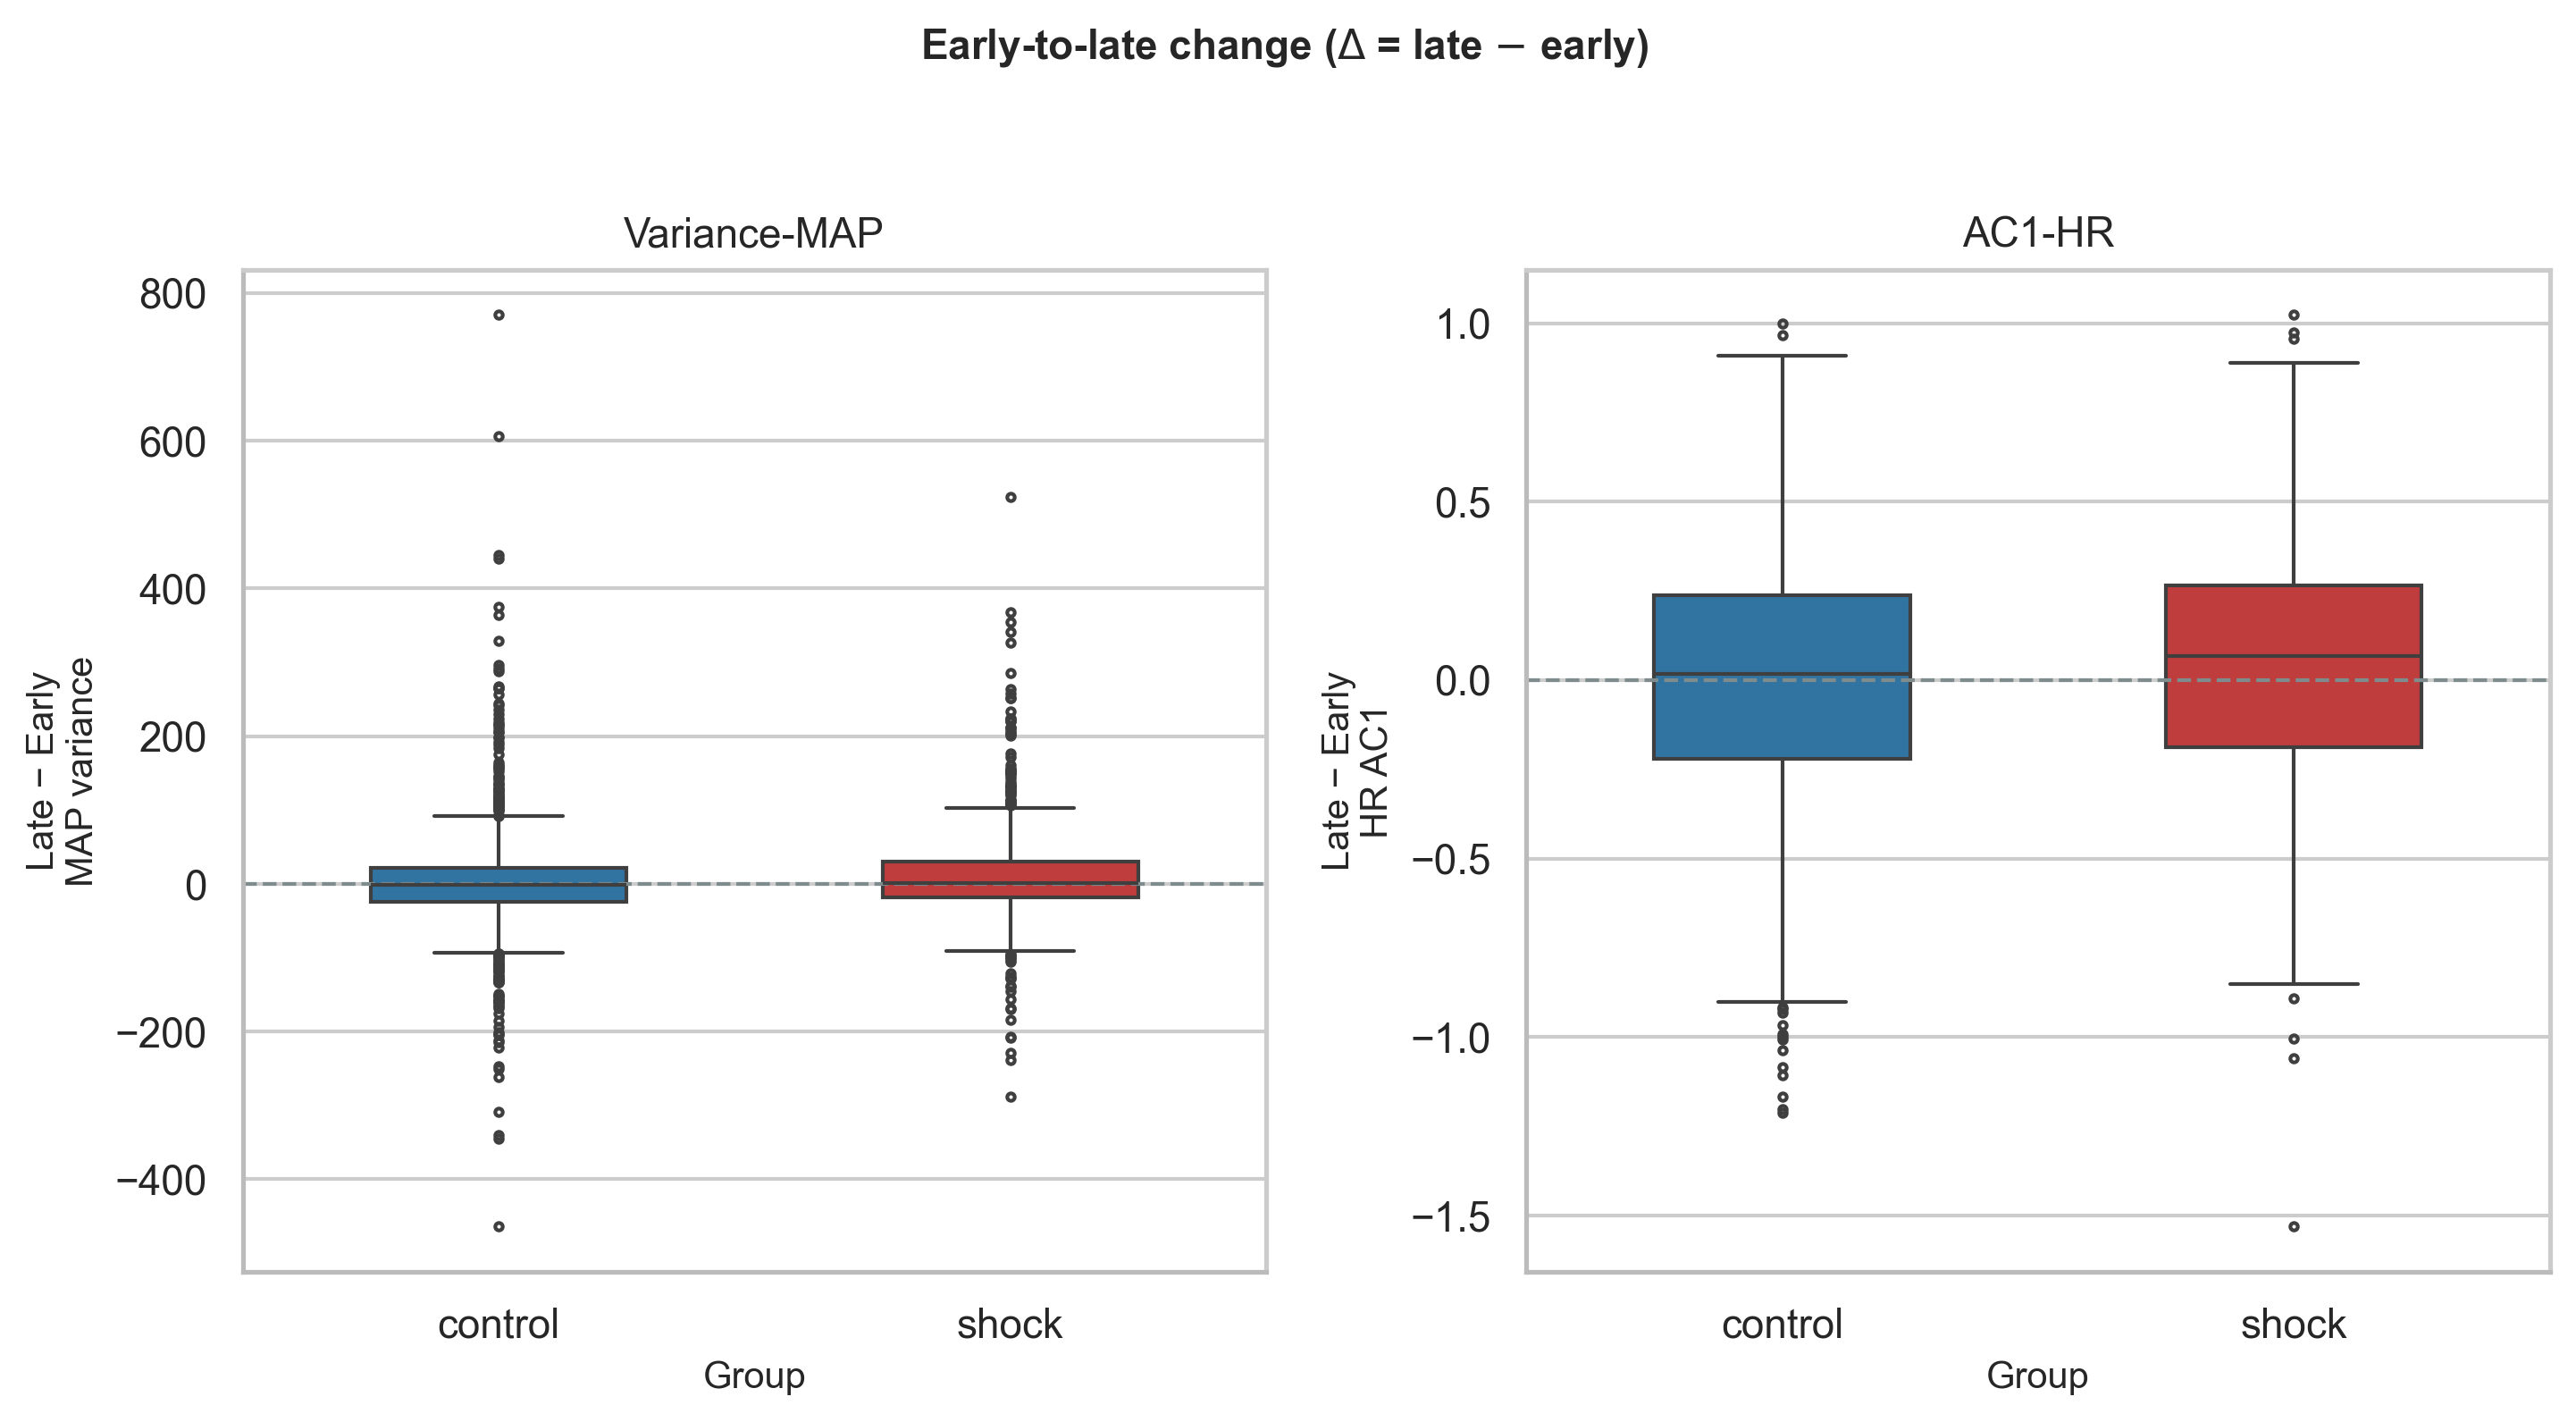
\includegraphics[width=\textwidth]{figures/figS3_delta_ac1.png}
    \caption{AC1 and MAP variance.}
  \end{subfigure}
  \hfill
  \begin{subfigure}[b]{0.48\textwidth}
    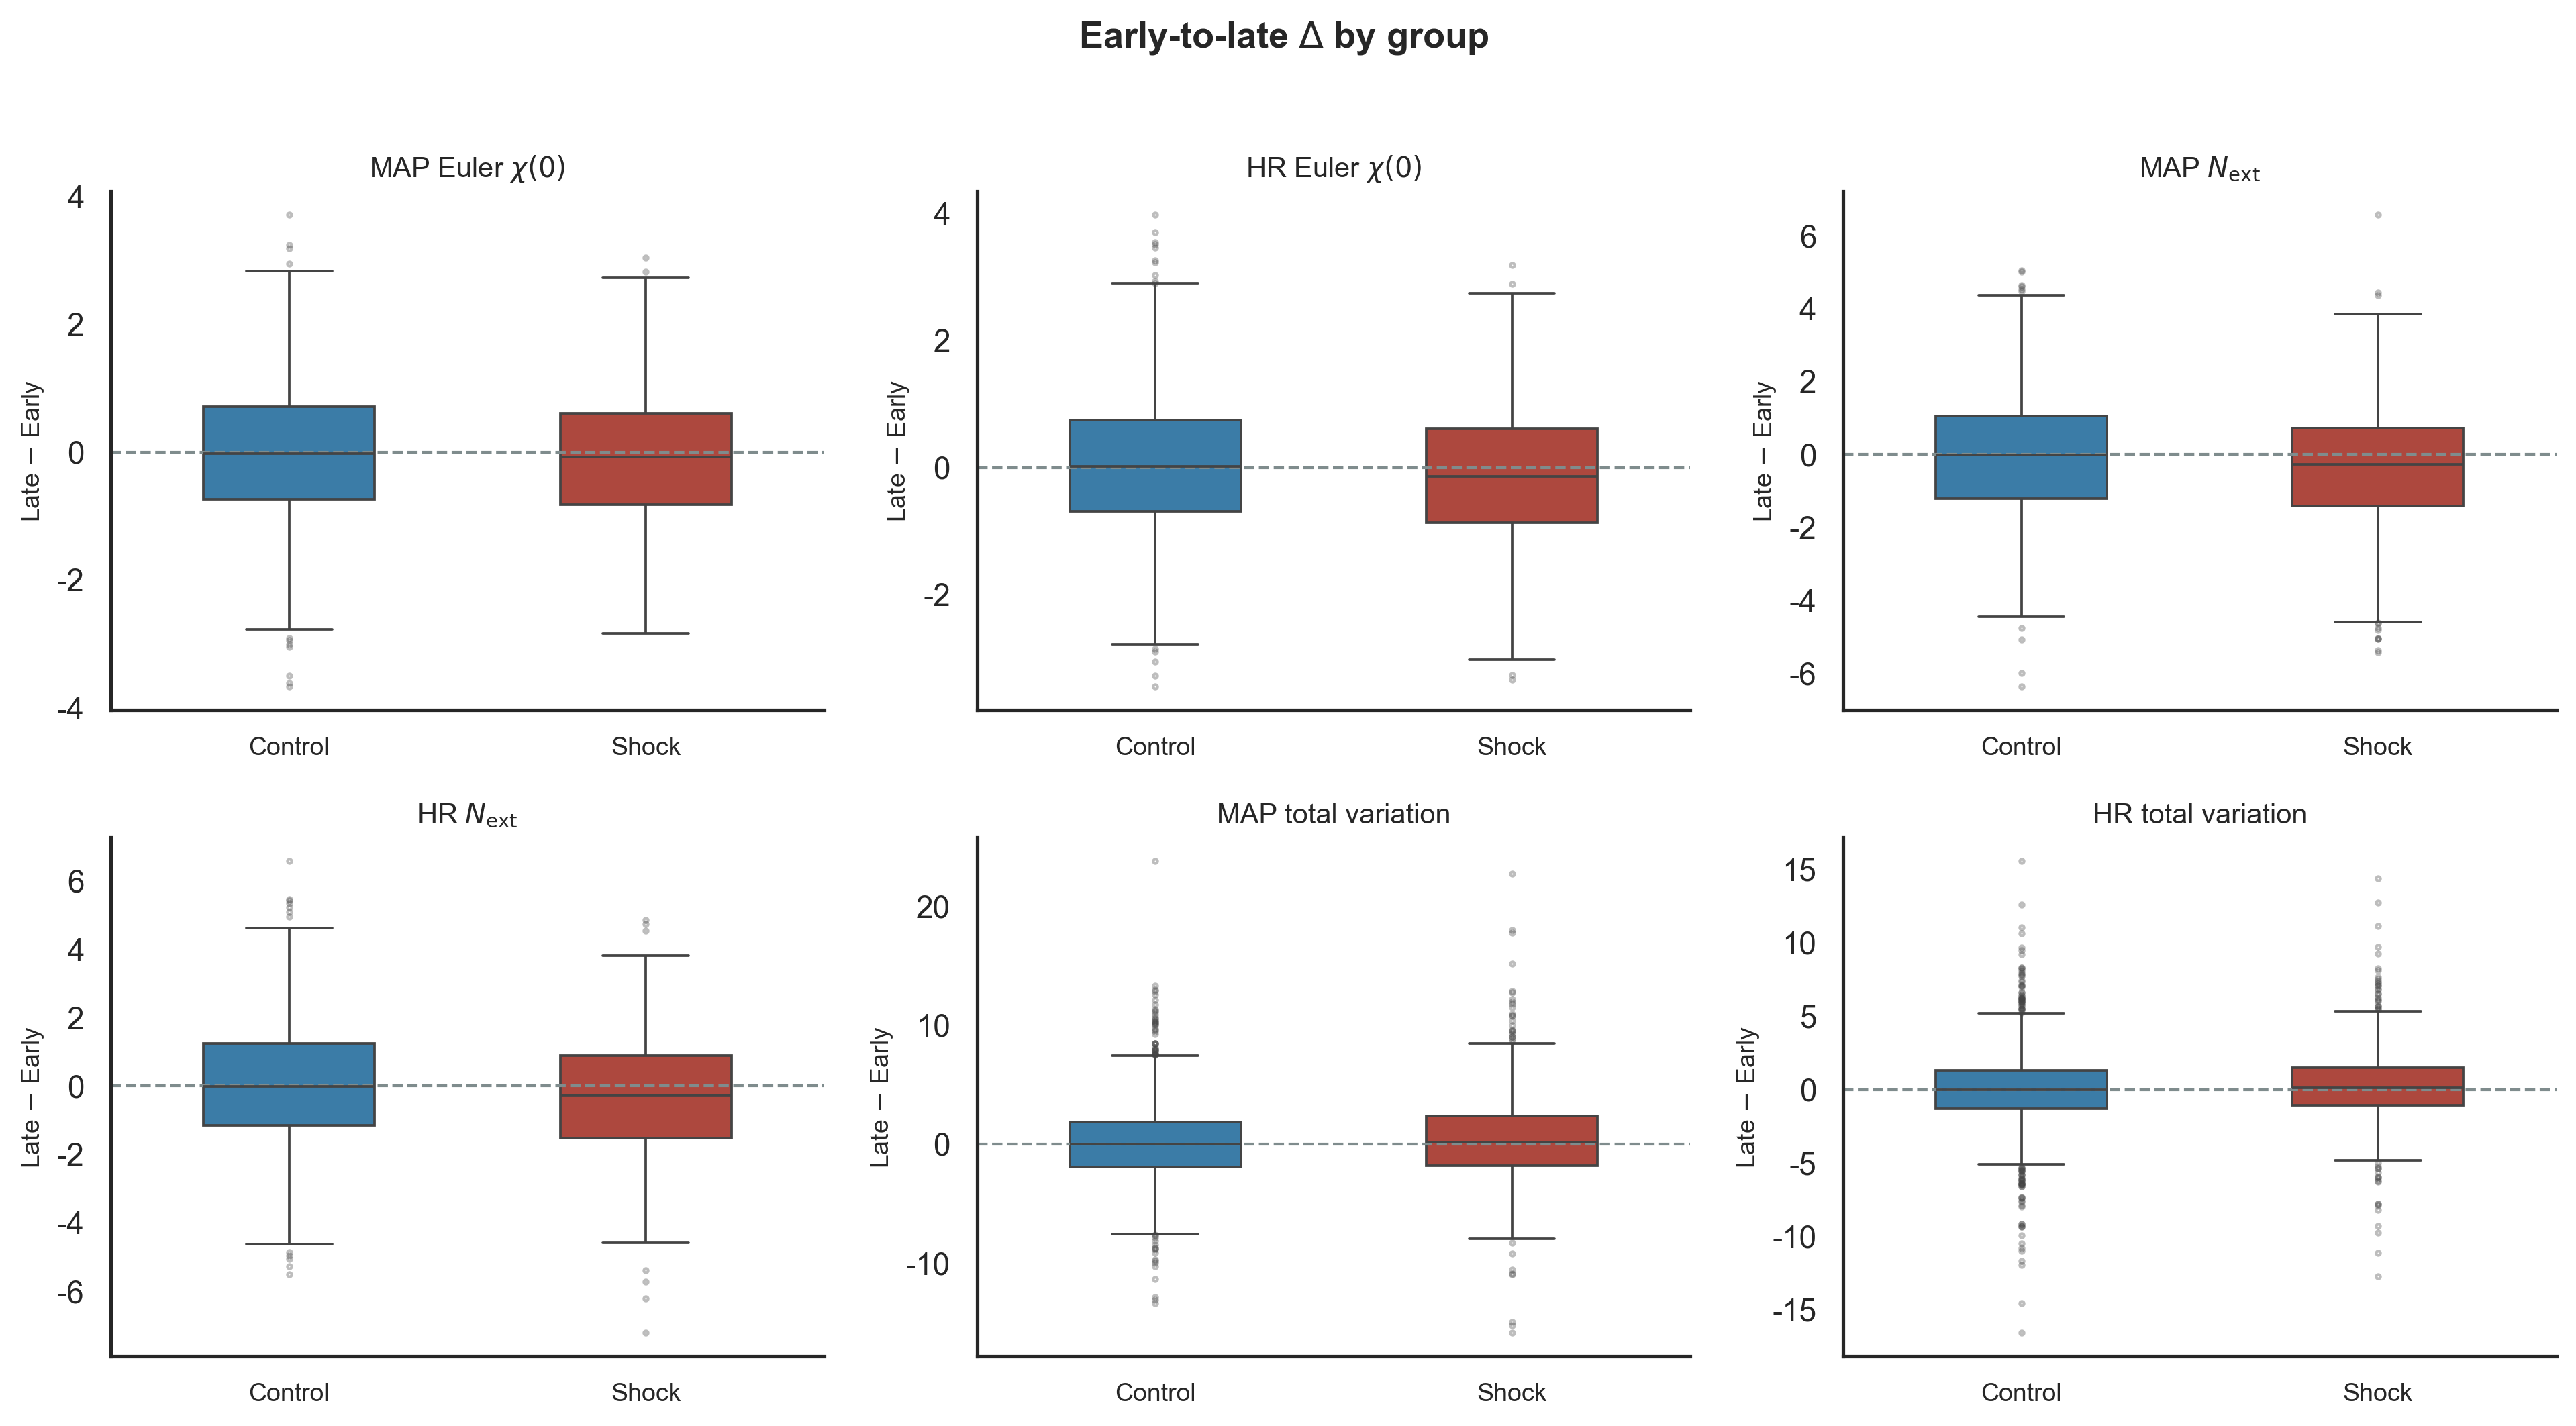
\includegraphics[width=\textwidth]{figures/figS3_delta_euler.png}
    \caption{Topological indicators.}
  \end{subfigure}
  \caption{Early-to-late change ($\Delta$ = late $-$ early) in
  early-warning indicators by group (shock vs control).
  Horizontal dashed line at 0.
  HR \chihr\ and HR \Nextreme\ show significantly more negative $\Delta$
  in the shock group (Holm $p\leq0.013$), indicating progressive loss of
  oscillatory complexity approaching shock onset.}
  \label{fig:delta}
\end{figure}

% Table S1: SOFA/APACHE independence (eICU)
\begin{table}[htbp]
  \centering
  \caption{Severity-score independence: conditional logistic regression
  adjusted for SOFA non-cardiovascular and APACHE-IVa in eICU-CRD
  ($T_0\geq72$\,h subset).}
  \label{tab:sofa}
  \small
  \begin{tabular}{llccc}
    \toprule
    \textbf{Indicator} & \textbf{Adjustment} & \textbf{OR (95\,\%\,CI)} & \textbf{$p$} & \textbf{Strata} \\
    \midrule
    \multicolumn{5}{l}{\textit{$T_0\geq72$\,h subset (103 pairs)}} \\
    $N_{\text{extrema}}$ & Alone              & 0.79 (0.64--0.97) & 0.023 & 100 \\
    $N_{\text{extrema}}$ & + SOFA non-cardio  & 0.80 (0.65--0.99) & 0.041 & 100 \\
    $N_{\text{extrema}}$ & + APACHE-IVa       & 0.77 (0.60--0.99) & 0.038 & 72 \\
    $\chi_{\text{HR}}(0)$ & Alone             & 0.72 (0.50--1.03) & 0.073 & 100 \\
    $\chi_{\text{HR}}(0)$ & + SOFA non-cardio & 0.75 (0.52--1.09) & 0.135 & 100 \\
    AC1 & Alone                               & 2.36 (0.81--6.83) & 0.114 & 100 \\
    AC1 & + SOFA non-cardio                   & 1.93 (0.65--5.75) & 0.237 & 100 \\
    \bottomrule
  \end{tabular}
  \vspace{2pt}\\
  \raggedright\footnotesize
  SOFA non-cardiovascular excludes the vasopressor-dependent cardiovascular
  sub-score (near-perfectly concordant with shock status by definition).
  APACHE strata reduced due to missing APACHE-IVa in some hospitals.
\end{table}

% Table S2: GEE + unconditional logistic + dedup sensitivity (AC1)
\begin{table}[htbp]
  \centering
  \caption{AC1 sensitivity analyses: GEE, unconditional logistic
  regression, and de-duplicated cohort (one admission per patient).}
  \label{tab:dedup}
  \small
  \begin{tabular}{lcc}
    \toprule
    \textbf{Analysis} & \textbf{OR (95\,\%\,CI)} & \textbf{$p$} \\
    \midrule
    \multicolumn{3}{l}{\textit{Alternative variance structures}} \\
    Standard logistic (adjusted)       & 1.63 (1.18--2.25) & 0.003 \\
    GEE logistic (adjusted)            & 1.61 (1.17--2.22) & 0.003 \\
    Conditional logistic (primary)     & 1.60 (1.15--2.22) & 0.005 \\
    \midrule
    \multicolumn{3}{l}{\textit{Deduplicated subset (one $T_0$ per stay)}} \\
    Conditional logistic ($N=1{,}915$) & 1.65 (1.18--2.31) & 0.003 \\
    \bottomrule
  \end{tabular}
\end{table}

% Table S3: Bootstrap CIs (AC1)
\begin{table}[htbp]
  \centering
  \caption{Bootstrap confidence intervals for AC1 conditional logistic
  regression (1,000 pair-stratified resamples).}
  \label{tab:bootstrap}
  \small
  \begin{tabular}{lccc}
    \toprule
    \textbf{Statistic} & \textbf{Observed $\Delta$} & \textbf{Bootstrap 95\,\%\,CI} & \textbf{Excludes 0} \\
    \midrule
    Late-window AC1 mean   & 0.0589 & [0.0331, 0.0862] & Yes \\
    Early-window AC1 mean  & 0.0221 & [0.0033, 0.0465] & Yes \\
    Early-to-late AC1 change & 0.0374 & [0.0041, 0.0647] & Yes \\
    \bottomrule
  \end{tabular}
  \vspace{2pt}\\
  \raggedright\footnotesize
  1,000 pair-stratified bootstrap resamples; percentile method CIs.
\end{table}

% Table S4: Double-detrending sensitivity
\begin{table}[htbp]
  \centering
  \caption{Double-detrending sensitivity analysis: AC1 results
  after additional within-window linear detrending.}
  \label{tab:doubledetrend}
  \small
  \begin{tabular}{lcc}
    \toprule
    \textbf{Variable} & \textbf{OR (95\,\%\,CI)} & \textbf{$p$} \\
    \midrule
    HR AC1, late window mean$^\dagger$ & 1.29 (0.91--1.83) & 0.159 \\
    Invasive MV at $-$12\,h       & 0.71 (0.56--0.90) & 0.005 \\
    Sedation exposure              & 4.70 (3.73--5.92) & $<$0.001 \\
    Beta-blocker exposure          & 0.66 (0.44--0.99) & 0.047 \\
    \bottomrule
  \end{tabular}
  \vspace{2pt}\\
  \raggedright\footnotesize
  $^\dagger$ Primary predictor.
  Double detrending: 24-h trailing mean $+$ within-window 12-h linear detrend.
  AC1 no longer significant, indicating sensitivity to detrending specification.
\end{table}

% Table S5: SampEn m=2 sensitivity
\begin{table}[htbp]
  \centering
  \caption{SampEn sensitivity analysis: $m=2$ (vs primary $m=1$),
  $r=0.5\sigma_{48}$.}
  \label{tab:sampenm2}
  \small
  \begin{tabular}{llccc}
    \toprule
    \textbf{Specification} & \textbf{Model} & \textbf{OR (95\,\%\,CI)} & \textbf{$p$} & \textbf{$N$} \\
    \midrule
    $m=1$, $r=0.5\sigma_{48}$ & M1 & 0.86 (0.69--1.07) & 0.178 & 2{,}122 \\
    $m=1$, $r=0.5\sigma_{48}$ & S1 & 0.81 (0.64--1.02) & 0.067 & 2{,}122 \\
    $m=1$, $r=0.5\sigma_{48}$ & S2 & 0.87 (0.68--1.12) & 0.284 & 2{,}104 \\
    \midrule
    $m=2$, $r=0.5\sigma_{48}$ & M1 & 0.84 (0.63--1.12) & 0.226 & 1{,}824 \\
    $m=2$, $r=0.5\sigma_{48}$ & S1 & 0.76 (0.56--1.02) & 0.066 & 1{,}824 \\
    $m=2$, $r=0.5\sigma_{48}$ & S2 & 0.78 (0.56--1.09) & 0.150 & 1{,}809 \\
    \bottomrule
  \end{tabular}
  \vspace{2pt}\\
  \raggedright\footnotesize
  Neither $m=1$ nor $m=2$ specification produces significant associations.
  Sample size reduction at $m=2$ reflects increased NaN rates from
  stricter template matching.
\end{table}

% Table S6: Lactate-restricted sensitivity analysis
\begin{table}[htbp]
  \centering
  \caption{Lactate-restricted sensitivity analysis (eICU-CRD).
  From the original 587 shock cases, 264 (45.6\%) had lactate
  $>$2\,mmol/L within $\pm$24\,h of \Tzero.
  Only matched pairs where the shock case met this criterion were retained
  (264 pairs, original matching preserved).
  M1: base conditional logistic model.}
  \label{tab:lactate-sens}
  \small
  \begin{tabular}{llcccc}
    \toprule
    & & \multicolumn{2}{c}{\textbf{Lactate-restricted}} &
      \multicolumn{2}{c}{\textbf{Original (all pairs)}} \\
    \cmidrule(lr){3-4} \cmidrule(lr){5-6}
    \textbf{Stratum} & \textbf{Metric} &
      \textbf{OR (95\,\%\,CI)} & \textbf{$p$} &
      \textbf{OR (95\,\%\,CI)} & \textbf{$p$} \\
    \midrule
    All (264 pairs)
      & AC1           & 0.85 (0.43--1.67) & 0.630  & 1.21 (0.75--1.97) & 0.435 \\
      & $N_{\text{extrema}}$ & 0.94 (0.83--1.07) & 0.381 & 0.94 (0.86--1.02) & 0.142 \\
      & Euler $\chi(0)$ & 0.96 (0.74--1.25) & 0.763 & 0.97 (0.81--1.16) & 0.756 \\
    \midrule
    $T_0\geq48$\,h (46 pairs)
      & AC1           & 1.08 (0.23--5.11) & 0.920  & 1.21 (0.50--2.93) & 0.673 \\
      & $N_{\text{extrema}}$ & 0.89 (0.64--1.25) & 0.506 & 0.92 (0.78--1.07) & 0.281 \\
      & Euler $\chi(0)$ & 0.81 (0.48--1.37) & 0.428 & 0.84 (0.62--1.14) & 0.262 \\
    \midrule
    $T_0\geq72$\,h (30 pairs)
      & AC1           & 0.67 (0.11--4.06) & 0.660  & 2.68 (0.88--8.12) & 0.082 \\
      & $N_{\text{extrema}}$ & 0.80 (0.51--1.26) & 0.334 & 0.80 (0.65--0.98) & 0.034 \\
      & Euler $\chi(0)$ & 0.89 (0.50--1.56) & 0.676 & 0.72 (0.50--1.04) & 0.084 \\
    \bottomrule
  \end{tabular}
  \vspace{2pt}\\
  \raggedright\footnotesize
  Point estimates for $N_{\text{extrema}}$ are identical at $T_0\geq72$\,h
  (OR\,=\,0.80 in both analyses); the loss of significance reflects reduced
  power (30 vs.\ 103 informative strata) rather than attenuation of effect size.
  The direction of association is consistent across all strata and metrics.
\end{table}

% ================================================================
\clearpage
\section*{Appendix: Mathematical Note on Euler Characteristic}
\label{app:math}
% SOURCE: euler_ews_medrxiv.tex Appendix (verbatim)

For a discrete one-dimensional signal
$r = (r_1, \ldots, r_n) \in \mathbb{R}^n$,
the \emph{sublevel set} at threshold $\lambda$ is
$S_\lambda = \{i \in \{1,\ldots,n\} : r_i \leq \lambda\}$,
viewed as a subset of the path graph on $n$ vertices.
The Euler characteristic of $S_\lambda$ is:
\[
  \chi(S_\lambda)
  = \beta_0(S_\lambda) - \beta_1(S_\lambda)
  = \beta_0(S_\lambda),
\]
since a subgraph of a path graph contains no cycles ($\beta_1 = 0$).
Here $\beta_0(S_\lambda)$ is the number of connected components;
for a path graph, these correspond to maximal contiguous runs of indices
with $r_i \leq \lambda$.

Setting $\lambda = 0$ (the detrended mean), $\chi_{\text{HR}}(0)$ counts
the number of below-mean oscillatory excursions.
This equals $N_{\text{extrema}}/2 + \varepsilon$ (where $\varepsilon \in \{0,1\}$
depends on boundary conditions), making the two indicators conceptually
complementary: $\chi_{\text{HR}}(0)$ is the topological count of
below-mean runs, while $N_{\text{extrema}}$ counts all direction reversals.

\end{document}
